\documentclass{article}
\usepackage[backend=biber]{biblatex}
\usepackage{graphicx}
\usepackage[]{hyperref}
\usepackage{graphicx}
\usepackage{svgcolor}
\usepackage{lscape}
\usepackage{booktabs}
\usepackage{longtable}
\usepackage{float}
\usepackage[table,xcdraw]{xcolor}
\usepackage{siunitx}
\usepackage[]{amsmath}
\usepackage{physics}
\usepackage{gensymb}
\usepackage{mathtools}
\usepackage{fancyref}

\addbibresource{/home/giorgio/Bibliography/bibliography.bib}
\hypersetup{
    colorlinks=true,
    linkcolor=blue,
    citecolor=blue,
    filecolor=magenta,      
    urlcolor=cyan,
    pdftitle={Relazione Veicoli Aerospaziali},
    bookmarks=true,
}
\author{Giorgio De Trane s275514}
\title{\textbf{RELAZIONE VEICOLI AEROSPAZIALI}}

\begin{document}
\setlength{\parindent}{0pt}
\maketitle
\begin{center}
    \textit{Anno accademico 2020-2021}
\end{center}
\begin{figure}[h!]
    \centering
    
\includegraphics[width=\textwidth]{Sources/Plots_and_Pictures/polito_logo.png}\\
\end{figure}
\pagebreak
\tableofcontents
\pagebreak
\section{Assignment 1\label{Assignment_1}}
\subsection{Assignment 1.1\label{Assignment_1.1}}

\textbf{Assignment}: Write down an initial list of requirements for an
aircraft that shall replace A350, with an entry into service in 2030.
Please, while listing the requirements, refer to the categories
reported in Sect.1.4
\newline
\newline
\textbf{\textit{List of Requirements}}\\\\ (Mainly based on Airbus A350-900 \autocite{Airbus_A350-900})
\\ 

\textbf{Design and Performance\label{Design_and_performance}}
\begin{itemize}
    \item Number of pilots: 2
    \item Cruise Mach: 0.85
    \item Max Operating Speed Mach: 0.9
    \item Cabin Crew: 8 (2 for each emergency exit)
    \item Number of passengers: 440
    \item Wing Span: under 70 m
    \item Fuselage Length: under 75 m
    \item Range: over 15000 km
    \item Height: under 18 m
    \item Wing Surface: 450 m²
    \item Max Payload: over 50 metric tonnes
    \item Number of engines: 2
\end{itemize}
\pagebreak
\textbf{Operational requirements\label{Operational_requirements}}
\begin{itemize}
    \item Cruise altitude: 10 - 13 km
    \item Turn around time: under 60 mins
    \item Takeoff distance: under 1 km
    \item Landing distance: under 2.5 km
    \item Rate of climb: 3000 ft/min (Initial climb)
    \item Ceiling: 13.15 km (FL431)
\end{itemize}

\textbf{Analysis of applicable regulations\label{Analysis_applicable_regulations}}
\begin{itemize}
    \item Number of exits: 8
    \item External noise (a terra a 5km di distanza) decollo: under 90 dB
    \item External noise (a terra a 5km di distanza) atterraggio: under 95 dB
    \item N max in condizioni operative: 2.5
    \item N min in condizioni operative: -1
\end{itemize}
\pagebreak
\subsection{Assignment 1.2\label{Assignment_1.2}}
\textbf{Assignment}: On the basis of the list of Requirements elicited
in the previous step, identify a good list of reference aircraft and
collect data to be used as meaningful statistical population.\\ \\ \\ 

Several commercial aicrafts from \textit{Airbus} and \textit{Boeing} have been chosen, with
the goal of having a statistical population to compare to in mind, as well as a reference list for 
inspiration with consolidated concept designs and technologies.\\
Acquiring all the data for the entire population was not easy, as their availability is scattered and varies from source
to source.\\
Despite the overall scarcity of clear, organized and transparent information, a significant amount of statistically meaningful
data has been acquired and ordered in the following landscape tables.\\ \\ 
A \textit{GNU/Octave} \autocite{Octave} (or Matlab) script that elaborates all the data has been written, with the goal
of easy readability in mind, as everything has been split into functions. \\
The script and its functions are publicly available in this works' \textit{GitHub} repository \autocite{Airbus_replacement_repo} (\textit{Code} directory) and 
licensed under the \textit{GNU GPL v3} license.\\ 
Bear in mind that Octave outputs all the plots at once when you run the whole script, while on Matlab
you may need to run each separate Section, as some versions overwrite \textit{figure()} when it's implemented
within a custom function.\\ 
This will of course depend on the Matlab version you're currently running.\\ The code itself is short and easy to read,
while also being full of step-by-step comments.


\newpage


\begin{landscape}
    \begin{table}[]
    \centering
    \resizebox{1.7\textwidth}{!}{%
    \begin{tabular}{@{}lccccccccccc@{}}
    \rowcolor[HTML]{FF7A7A} 
    \cellcolor[HTML]{FFC99B}Design \& Performance parameters &
      \multicolumn{1}{l}{\cellcolor[HTML]{FF7A7A}B787-10 Dre} &
      \multicolumn{1}{l}{\cellcolor[HTML]{FF2C2C}A350 XWB-900} &
      \multicolumn{1}{l}{\cellcolor[HTML]{FF7A7A}A330 Neo -900} &
      \multicolumn{1}{l}{\cellcolor[HTML]{FF7A7A}B777-300ER} &
      \multicolumn{1}{l}{\cellcolor[HTML]{FF7A7A}B777 X-900} &
      \multicolumn{1}{l}{\cellcolor[HTML]{FF7A7A}B787-8} &
      \multicolumn{1}{l}{\cellcolor[HTML]{FF7A7A}A340-500} &
      \multicolumn{1}{l}{\cellcolor[HTML]{FF7A7A}A330-300} &
      \multicolumn{1}{l}{\cellcolor[HTML]{FF7A7A}A340-600} &
      \multicolumn{1}{l}{\cellcolor[HTML]{FF7A7A}A330-200} &
      \multicolumn{1}{l}{\cellcolor[HTML]{FF7A7A}B767-300} \\
    \rowcolor[HTML]{EFEFEF} 
    \cellcolor[HTML]{FFEF98}Number of pilots                & 2     & 2     & 2     & 2     & 2     & 2      & 2     & 2     & N.A.  & 2    & 2    \\
    \cellcolor[HTML]{FCF1B3}Cruise Mach number              & 0.85  & 0.85  & 0.81  & 0.84  & 0.84  & 0.85   & 0.83  & 0.86  & N.A.  & 0.86 & 0.86 \\
    \rowcolor[HTML]{EFEFEF} 
    \cellcolor[HTML]{FFEF98}Max Operating Speed Mach        & N.A.  & N.A.  & N.A.  & N.A.  & N.A.  & N.A.   & N.A.  & N.A.  & N.A.  & N.A. & N.A. \\
    \cellcolor[HTML]{FCF1B3}Cabin Crew                      & 8-9   & 8-9   & 8-9   & 14    & N.A.  & N.A.   & N.A.  & N.A.  & N.A.  & N.A. & N.A. \\
    \rowcolor[HTML]{EFEFEF} 
    \cellcolor[HTML]{FFEF98}Number of passengers            & 330   & 440   & 440   & 550   & 426   & 359    & 375   & 275   & N.A.  & N.A. & N.A. \\
    \cellcolor[HTML]{FCF1B3}Wing Span {[}m²{]}              & 60.81 & 64.75 & 64    & 64.8  & 72.8  & 60.12  & 60.3  & N.A.  & N.A.  & N.A. & N.A. \\
    \rowcolor[HTML]{EFEFEF} 
    \cellcolor[HTML]{FFEF98}Fuselage Length {[}m{]}         & 68    & 66.8  & 63.66 & 73.86 & 76.72 & 56.72  & 67.93 & N.A.  & N.A.  & N.A. & N.A. \\
    \cellcolor[HTML]{FCF1B3}Range {[}km{]}                  & 11750 & 15000 & 13334 & 13650 & 13500 & 13620  & 12400 & 11750 & 14450 & N.A. & N.A. \\
    \rowcolor[HTML]{EFEFEF} 
    \cellcolor[HTML]{FFEF98}Wing Surface {[}m²{]}           & 377   & 443   & 465   & 436.8 & 516.7 & 377    & 437.3 & N.A.  & N.A.  & N.A. & N.A. \\
    \cellcolor[HTML]{FCF1B3}Height {[}m{]}                  & 17.02 & 17.47 & 16.79 & 18.76 & 19.53 & 16.92  & 17.53 & N.A.  & N.A.  & N.A. & N.A. \\
    \rowcolor[HTML]{EFEFEF} 
    \cellcolor[HTML]{FFEF98}Max Payload {[}metric tonnes{]} & 57    & 53    & 44    & 69.8  & 73.5  & 43.318 & 54    & N.A.  & N.A.  & N.A. & N.A. \\
    \cellcolor[HTML]{FCF1B3}Number of engines               & 2     & 2     & 2     & 2     & 2     & 2      & 4     & N.A.  & N.A.  & N.A. & N.A.
    \end{tabular}%
    }
    \caption{Statistical Population - Design and Performance parameters}
    \label{tab:stat_pop_des_perf}
    \end{table}
\end{landscape}

    \clearpage
    \newpage

\begin{landscape}
    \begin{table}[]
    \centering
    \resizebox{1.7\textwidth}{!}{%
    \begin{tabular}{@{}lccccccccccc@{}}
    \rowcolor[HTML]{FF7A7A} 
    \cellcolor[HTML]{FFC99B}Operational requirements &
      \multicolumn{1}{l}{\cellcolor[HTML]{FF7A7A}B787-10 Dre} &
      \multicolumn{1}{l}{\cellcolor[HTML]{FF2C2C}A350 XWB-900} &
      \multicolumn{1}{l}{\cellcolor[HTML]{FF7A7A}A330 Neo -900} &
      \multicolumn{1}{l}{\cellcolor[HTML]{FF7A7A}B777-300ER} &
      \multicolumn{1}{l}{\cellcolor[HTML]{FF7A7A}B777 X-900} &
      \multicolumn{1}{l}{\cellcolor[HTML]{FF7A7A}B787-8} &
      \multicolumn{1}{l}{\cellcolor[HTML]{FF7A7A}A340-500} &
      \multicolumn{1}{l}{\cellcolor[HTML]{FF7A7A}A330-300} &
      \multicolumn{1}{l}{\cellcolor[HTML]{FF7A7A}A340-600} &
      \multicolumn{1}{l}{\cellcolor[HTML]{FF7A7A}A330-200} &
      \multicolumn{1}{l}{\cellcolor[HTML]{FF7A7A}B767-300} \\
    \rowcolor[HTML]{EFEFEF} 
    \cellcolor[HTML]{FFEF98}Cruise altitude {[}m{]}    & N.A.  & N.A.   & N.A.  & N.A.  & 13136.88 & N.A.  & N.A.  & N.A. & N.A. & N.A. & N.A. \\
    \cellcolor[HTML]{FCF1B3}Turn around time {[}min{]} & 44    & 34 -62 & N.A.  & 30    & N.A.     & N.A.  & N.A.  & N.A. & N.A. & N.A. & N.A. \\
    \rowcolor[HTML]{EFEFEF} 
    \cellcolor[HTML]{FFEF98}Takeoff distance {[}m{]}   & 2600  & N.A.   & N.A.  & N.A.  & N.A.     & 2600  & 13350 & N.A. & N.A. & N.A. & N.A. \\
    \cellcolor[HTML]{FCF1B3}Landing distance {[}m{]}   & 2000  & N.A.   & N.A.  & N.A.  & N.A.     & N.A.  & N.A.  & N.A. & N.A. & N.A. & N.A. \\
    \rowcolor[HTML]{EFEFEF} 
    \cellcolor[HTML]{FFEF98}Rate of climb              & N.A.  & N.A.   & N.A.  & N.A.  & N.A.     & N.A.  & N.A.  & N.A. & N.A. & N.A. & N.A. \\
    \cellcolor[HTML]{FCF1B3}Ceiling {[}m{]}            & 13136 & 13100  & 12634 & 13136 & 13140    & 13100 & 12634 & N.A. & N.A. & N.A. & N.A.
    \end{tabular}%
    }
    \caption{Statistical Population - Operational Requirements}
    \label{tab:stat_pop_op_req}
    \end{table}
    \end{landscape}
    \clearpage


\begin{landscape}
    \begin{table}[]
    \centering
    \resizebox{1.7\textwidth}{!}{%
    \begin{tabular}{@{}lccccccccccc@{}}
    \rowcolor[HTML]{FF7A7A} 
    \cellcolor[HTML]{FFC99B}\textbf{Weights, Fuel and Aerodynamics} &
      \multicolumn{1}{l}{\cellcolor[HTML]{FF7A7A}B787-10 Dre} &
      \multicolumn{1}{l}{\cellcolor[HTML]{FF2C2C}A350 XWB-900} &
      \multicolumn{1}{l}{\cellcolor[HTML]{FF7A7A}A330 Neo -900} &
      \multicolumn{1}{l}{\cellcolor[HTML]{FF7A7A}B777-300ER} &
      \multicolumn{1}{l}{\cellcolor[HTML]{FF7A7A}B777 X-900} &
      \multicolumn{1}{l}{\cellcolor[HTML]{FF7A7A}B787-8} &
      \multicolumn{1}{l}{\cellcolor[HTML]{FF7A7A}A340-500} &
      \multicolumn{1}{l}{\cellcolor[HTML]{FF7A7A}A330-300} &
      \multicolumn{1}{l}{\cellcolor[HTML]{FF7A7A}A340-600} &
      \multicolumn{1}{l}{\cellcolor[HTML]{FF7A7A}A330-200} &
      \multicolumn{1}{l}{\cellcolor[HTML]{FF7A7A}B767-300} \\
    \rowcolor[HTML]{EFEFEF} 
    \cellcolor[HTML]{FFEF98}MTOW {[}kg{]}           & 250000 & 275000 & 251000 & 351535 & 352000 & 227940 & 365000 & 242000 & 380000 & 230000 & 158758 \\
    \cellcolor[HTML]{FCF1B3}Fuel Mass {[}kg{]}      & 101456 & 110523 & 111272 & 146839 & 160000 & 101323 & 110400 & N.A.   & N.A.   & N.A.   & N.A.   \\
    \rowcolor[HTML]{EFEFEF} 
    \cellcolor[HTML]{FFEF98}Empty Weight {[}kg{]}   & 135500 & 142400 & 137000 & 167829 & 181400 & 119950 & 177755 & 109400 & 174000 & 120600 & 86069  \\
    \cellcolor[HTML]{FCF1B3}Allungamento Alare      & 10.03  & 9.49   & 11     & 9.82   & 9.96   & 9.59   & 9.3    & N.A.   & N.A.   & N.A.   & N.A.   \\
    \rowcolor[HTML]{EFEFEF} 
    \cellcolor[HTML]{FFEF98}Cruise Speed {[}km/h{]} & 1050   & 903    & 918    & 905    & 900    & 903    & 871    & N.A.   & N.A.   & N.A.   & N.A.   \\
    \cellcolor[HTML]{FCF1B3}L/D                     & 20     & 21     & N.A.   & N.A.   & N.A.   & 21.23  & 16.2   & N.A.   & N.A.   & N.A.   & N.A.   \\
    \rowcolor[HTML]{EFEFEF} 
    \cellcolor[HTML]{FFEF98}SFC {[}lb/lbh{]}        & 0.506  & 0.478  & 0.506  & 0.56   & 0.545  & N.A.   & N.A.   & N.A.   & N.A.   & N.A.   & N.A.  
    \end{tabular}%
    }
    \caption{Statistical Population - Weights, Fuel and Aerodynamics}
    \label{tab:stat_pop_weight}
    \end{table}
    \end{landscape}
    \clearpage

\subsection{Assignment 1.3\label{Assignment_1.3}}
\textbf{Assignment}: \textit{Critical Analysis of statistical trends}.
Verify whether your statistical population fits the trend reported in
literature (e.g. Raymer) or suggest improvements to the simple
mathematical models (e.g. updates of coefficients).\\ \\ \\ 

Among all of the acquired data, the \textit{Empty Mass Fraction} is a particularly significant
statistical trend. \\
The raw data trend has been comparatively plot in the script, along with an improved algorithm, 
proposed by \textit{Daniel P. Raymer} \autocite{Raymer_Daniel}.

\begin{figure}[h!]
    \phantomsection
    \centering
    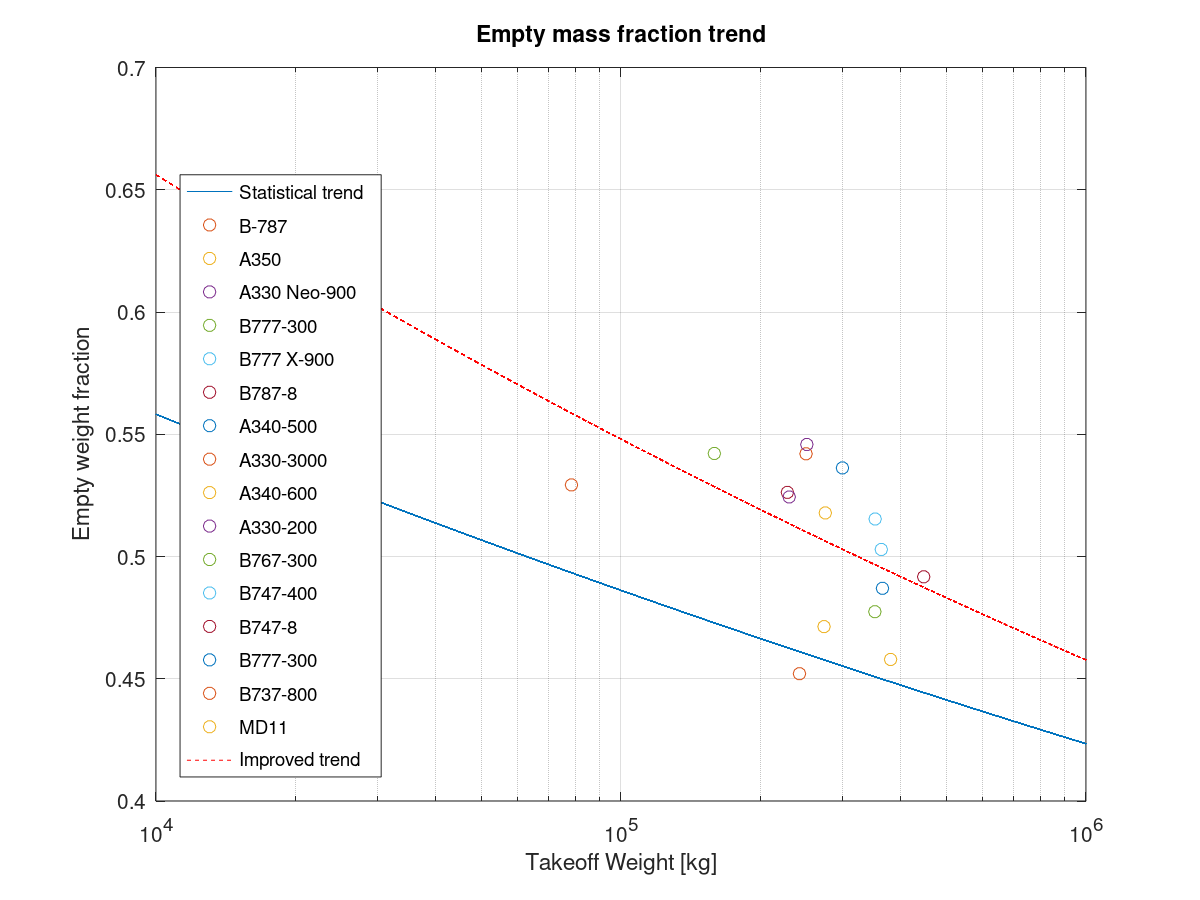
\includegraphics[width=\textwidth]{Sources/Plots_and_Pictures/Empty_mass_trend.png}\\
    \label{Empty_mass_trend}
    \caption{\textit{Empty Mass Trend}}
\end{figure} 

As clearly visible, the improved trend is substantially more in line with the acquired data.


\pagebreak
\subsection{Assignment 1.4\label{Assignments_1.4}}
\textbf{Assignment}: \textit{Guess data estimation for the reference
case study}. Apply the original or improved statistical trends to
perform the first guess data estimation for the reference case
study. Please, report all iterations needed to converge to the
design maximum take-off mass.\\ \\ \\ 

The first hypothesis for the \textit{MTOW} estimation was using the \textit{True Air Speed}
at an altitude of 10 km, as that would be a worse case scenario compared to the goal design
of a cruise Mach of 0.85. \\ 
The entire calculation is made assuming a range of 11 km and a maximum range of 15 km, as well as
a 50 metric tonnes design payload, with the awareness that a lighter payload might be necessary
in order to improve range.\\ \\
The function \begin{verbatim} mtow_range_plotter.m \end{verbatim} takes a guess \textit{MTOW} value as one of its inputs, generates some mass coefficients,
elaborates and uses them to finally return the desired \textit{MTOW} as one of its outputs (see repository \autocite{Airbus_replacement_repo} for the implementation).\\ 
The function also plots the MTOW as a function of the range.\\
One issue that has been immediately noticed is an instability with the plot around 15000 km,
therefore a compromise payload of 40 metric tonnes has been used for this specific plot, in order to 
get a more accurate visualization. \\ 
\begin{figure}[h!]
    \centering
    \phantomsection
    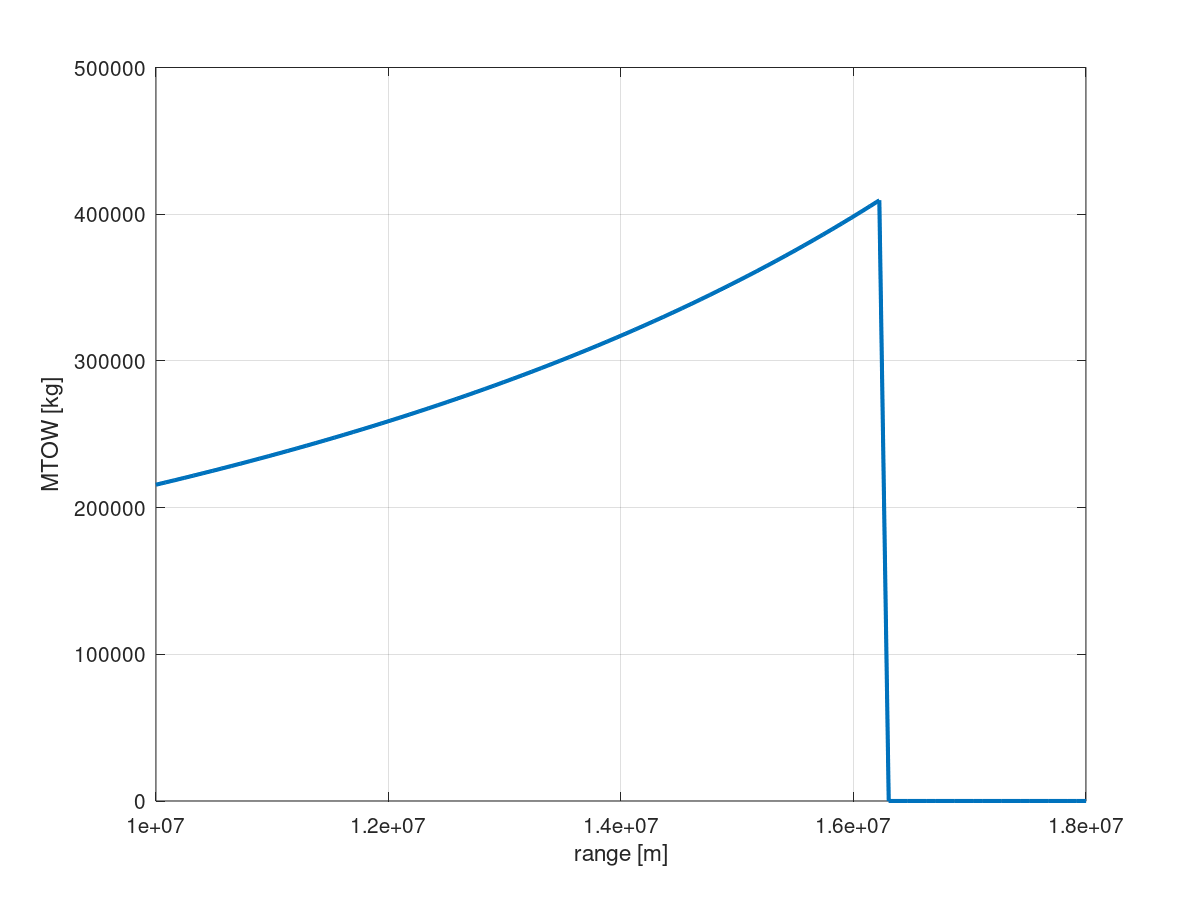
\includegraphics[width=0.7\textwidth]{Sources/Plots_and_Pictures/MTOW_range.png}
    \label{MTOW_Range}
    \caption{MTOW-Range}
\end{figure}
\clearpage
Similarly, with the function \autocite{Airbus_replacement_repo}
\begin{verbatim}

    mtow_payload_plotter.m

\end{verbatim}
the \textit{MTOW} has been plotted as a function of the payload with the design
range of 11000 km first, then with the maximum range of 15000 km, as pictured below.

\begin{figure}[h!]
    \centering
    \phantomsection
    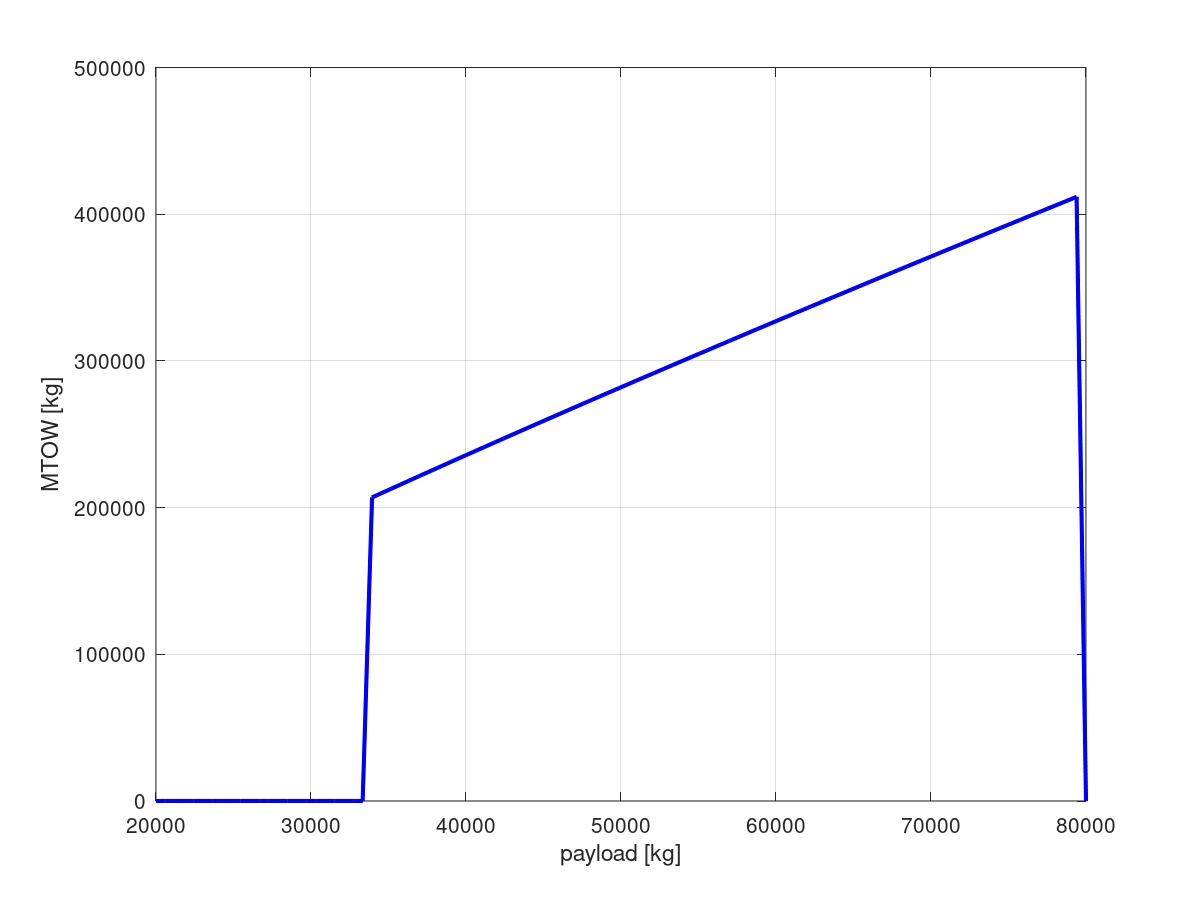
\includegraphics[width=\textwidth]{Sources/Plots_and_Pictures/MTOW_payload.png}
    \label{MTOW_Payload_11}
    \caption{MTOW-Payload (11000 km)}
\end{figure}
\clearpage
\begin{figure}[h!]
    \centering
    \phantomsection
    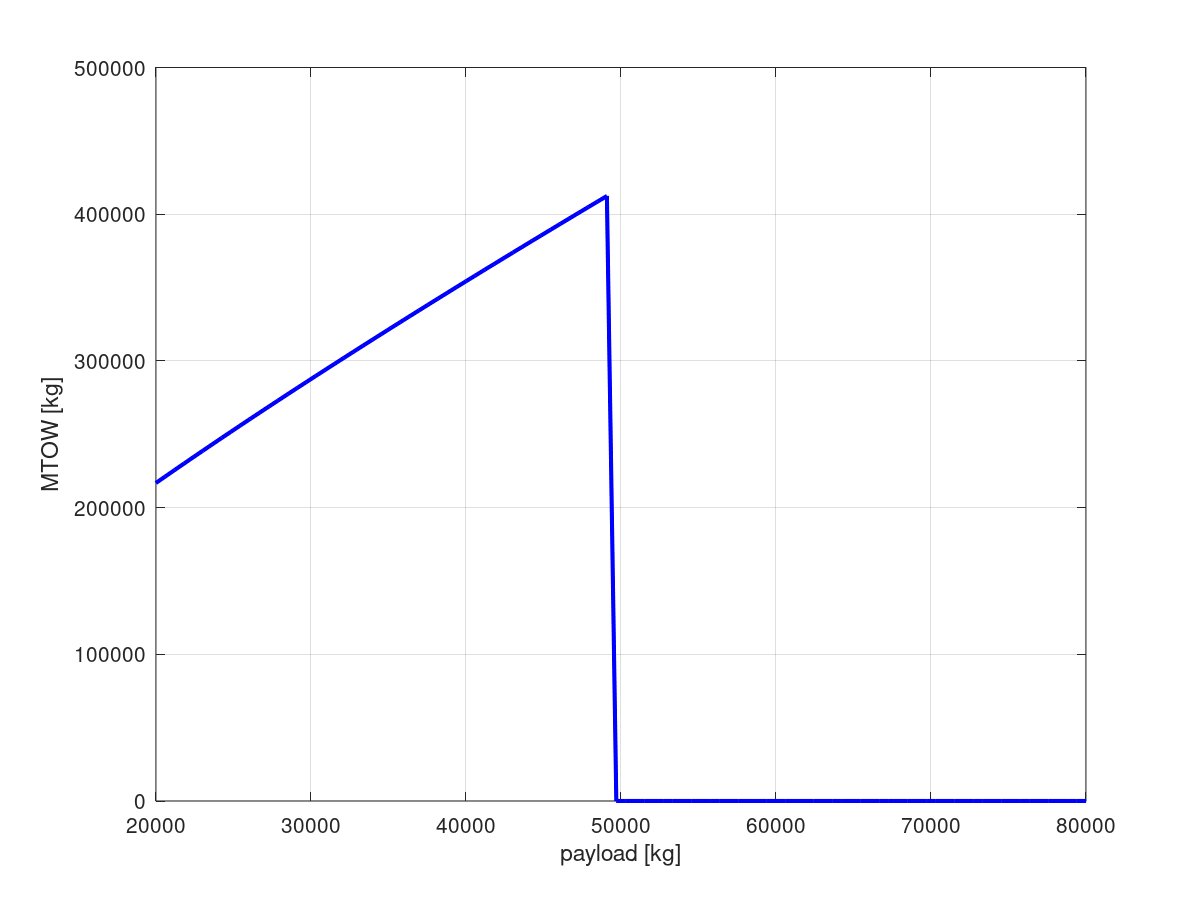
\includegraphics[width=\textwidth]{Sources/Plots_and_Pictures/MTOW_payload_2.png}
    \label{MTOW_Payload_15}
    \caption{MTOW-Payload (15000 km)}
\end{figure}
As you can see, there are areas where the function drops to a null value,
but that's because the MTOW ceases to have a physical meaning above or below certain
thresholds, depending on the input parameters. \\ 
However there seems to be a convergence slightly above 40 metric tonnes.
\clearpage

\section{Assignment 2\label{Assignment_2}}
\subsection{Assignment 2.1 and 2.2\label{Assignment_2.1}}
\textbf{Assignment:} Perform a Tradeoff and identify a suitable design point that 
guarantees the aircraft concept to be competitive with A350 and competitors. \\ \\ \\ 
\textbf{Assignment:} Create a Payload-Range Diagram representative of your aircraft concept. 
On the basis of the results achieved, draw different Payload-Range diagrams to explore 
the possibility to create a family concept.\\ \\ \\ 


Another key aspect to take into consideration is how the \textit{Payload} changes with 
 range, considering that fuel contribution to the total mass is obviously going
to change over time, thus influencing other factors as well. \\ 
The fuel volume of the Airbus A350 ($141 \ m^3$) as well as
the fuel itself (\textit{AVGAS}) have been taken as a reference point.\\ 
In order to better represent this function within a family of aircrafts that
is compatible with our statistical sample, a variation around the design point values has been 
taken into account.\\ 

\begin{itemize}
    \item Payload variation: $\pm \ 5000 \ kg$
    \item MTOW variation: $\left \{ {0.88 \ MTOW, 1.077 \ MTOW} \right \} \ kg$
    \item Range variation: $\pm \ 500 \ km$
\end{itemize}

The result is calculated and plotted with the function \autocite{Airbus_replacement_repo}
\begin{verbatim}
    payload_range_plotter.m
\end{verbatim}
which takes into consideration all the parameters involving the fuel, as well as other design values for the airplane.\\ 
The plotter can be called with input variations as many times as the user needs, while the `\textit{On}' parameter
is passed. \\ 
Finally, when the `\textit{Off}' parameter is passed, all the cases are plot on a single figure, with 
a randomized color palette.
\begin{figure}[h!]
    \phantomsection
    \centering
    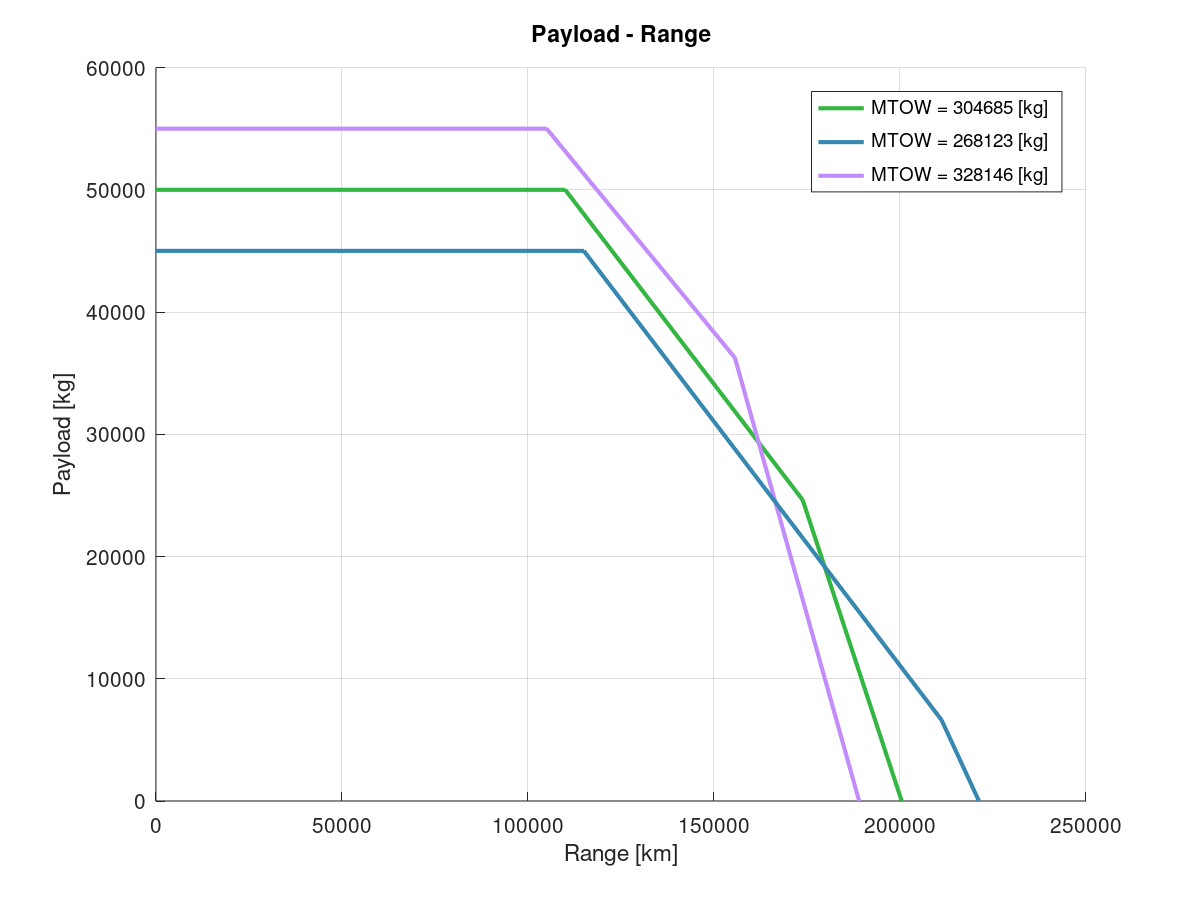
\includegraphics[width=\textwidth]{Sources/Plots_and_Pictures/Payload_range.png}
    \label{Payload_Range}
    \caption{Payload Range}
\end{figure}
\clearpage

As expected, the same fuel conditions for each sample case will produce the same slopes for each segment; moreover a higher
payload implies a higher MTOW (provided that all other factors are equalized), which in turn will reduce total range.\\ 
More precisely, the surface subtended by each segment defines three different areas (from left to right respectively) [\ref{Payload_Range}]:
\begin{itemize}
    \item Maximum payload
    \item Tradeoff between fuel and payload
    \item Tradeoff between payload and range
\end{itemize}

With a maximum design range of 15000 km and a starting payload of 50 metric tonnes, 
the designed aircraft is in an area where there needs to be a tradeoff between fuel and payload.\\ 
In order to achieve that range, some payload capacity needs to be sacrificed for more fuel.\\ 
However, with a minimum goal range of 11000 km, there is still is a chance to use the highest payload possible,
while increasing fuel, as that range falls within the first segment area. \\ 
It turns out that even the Airbus A350-900 XWB (which is the target retiring aircraft) declares
a maximum range of 15000 km; however, this range is not reached at maximum payload \autocite{Airbus_A350-900}.

\pagebreak
\subsection{Assignment 2.3\label{Assignment_2.3}}
\textbf{Assignment:} Once the maximum range requirement is refined,
 identify a set of city-pairs that can be connected with no-stop flight. \\ \\ \\ 

Using an opensource tool \autocite{OSM_radius_plotter} that can plot a circle on a map, given a certain radius, and having
Rome's Fiumicino Airport as a reference point, it's clearly visible from the picture below that both the 11000 km and the 15000 km ranges
can cover a substantial portion of the globe.\\ 
The tool used is based on Open Street Map \autocite{Open_Street_Map} and Leaflet \autocite{Leaflet}, a Javascript library
designed for maps generation and development. \\ 

\begin{figure}[h!]
    \phantomsection
    \centering
    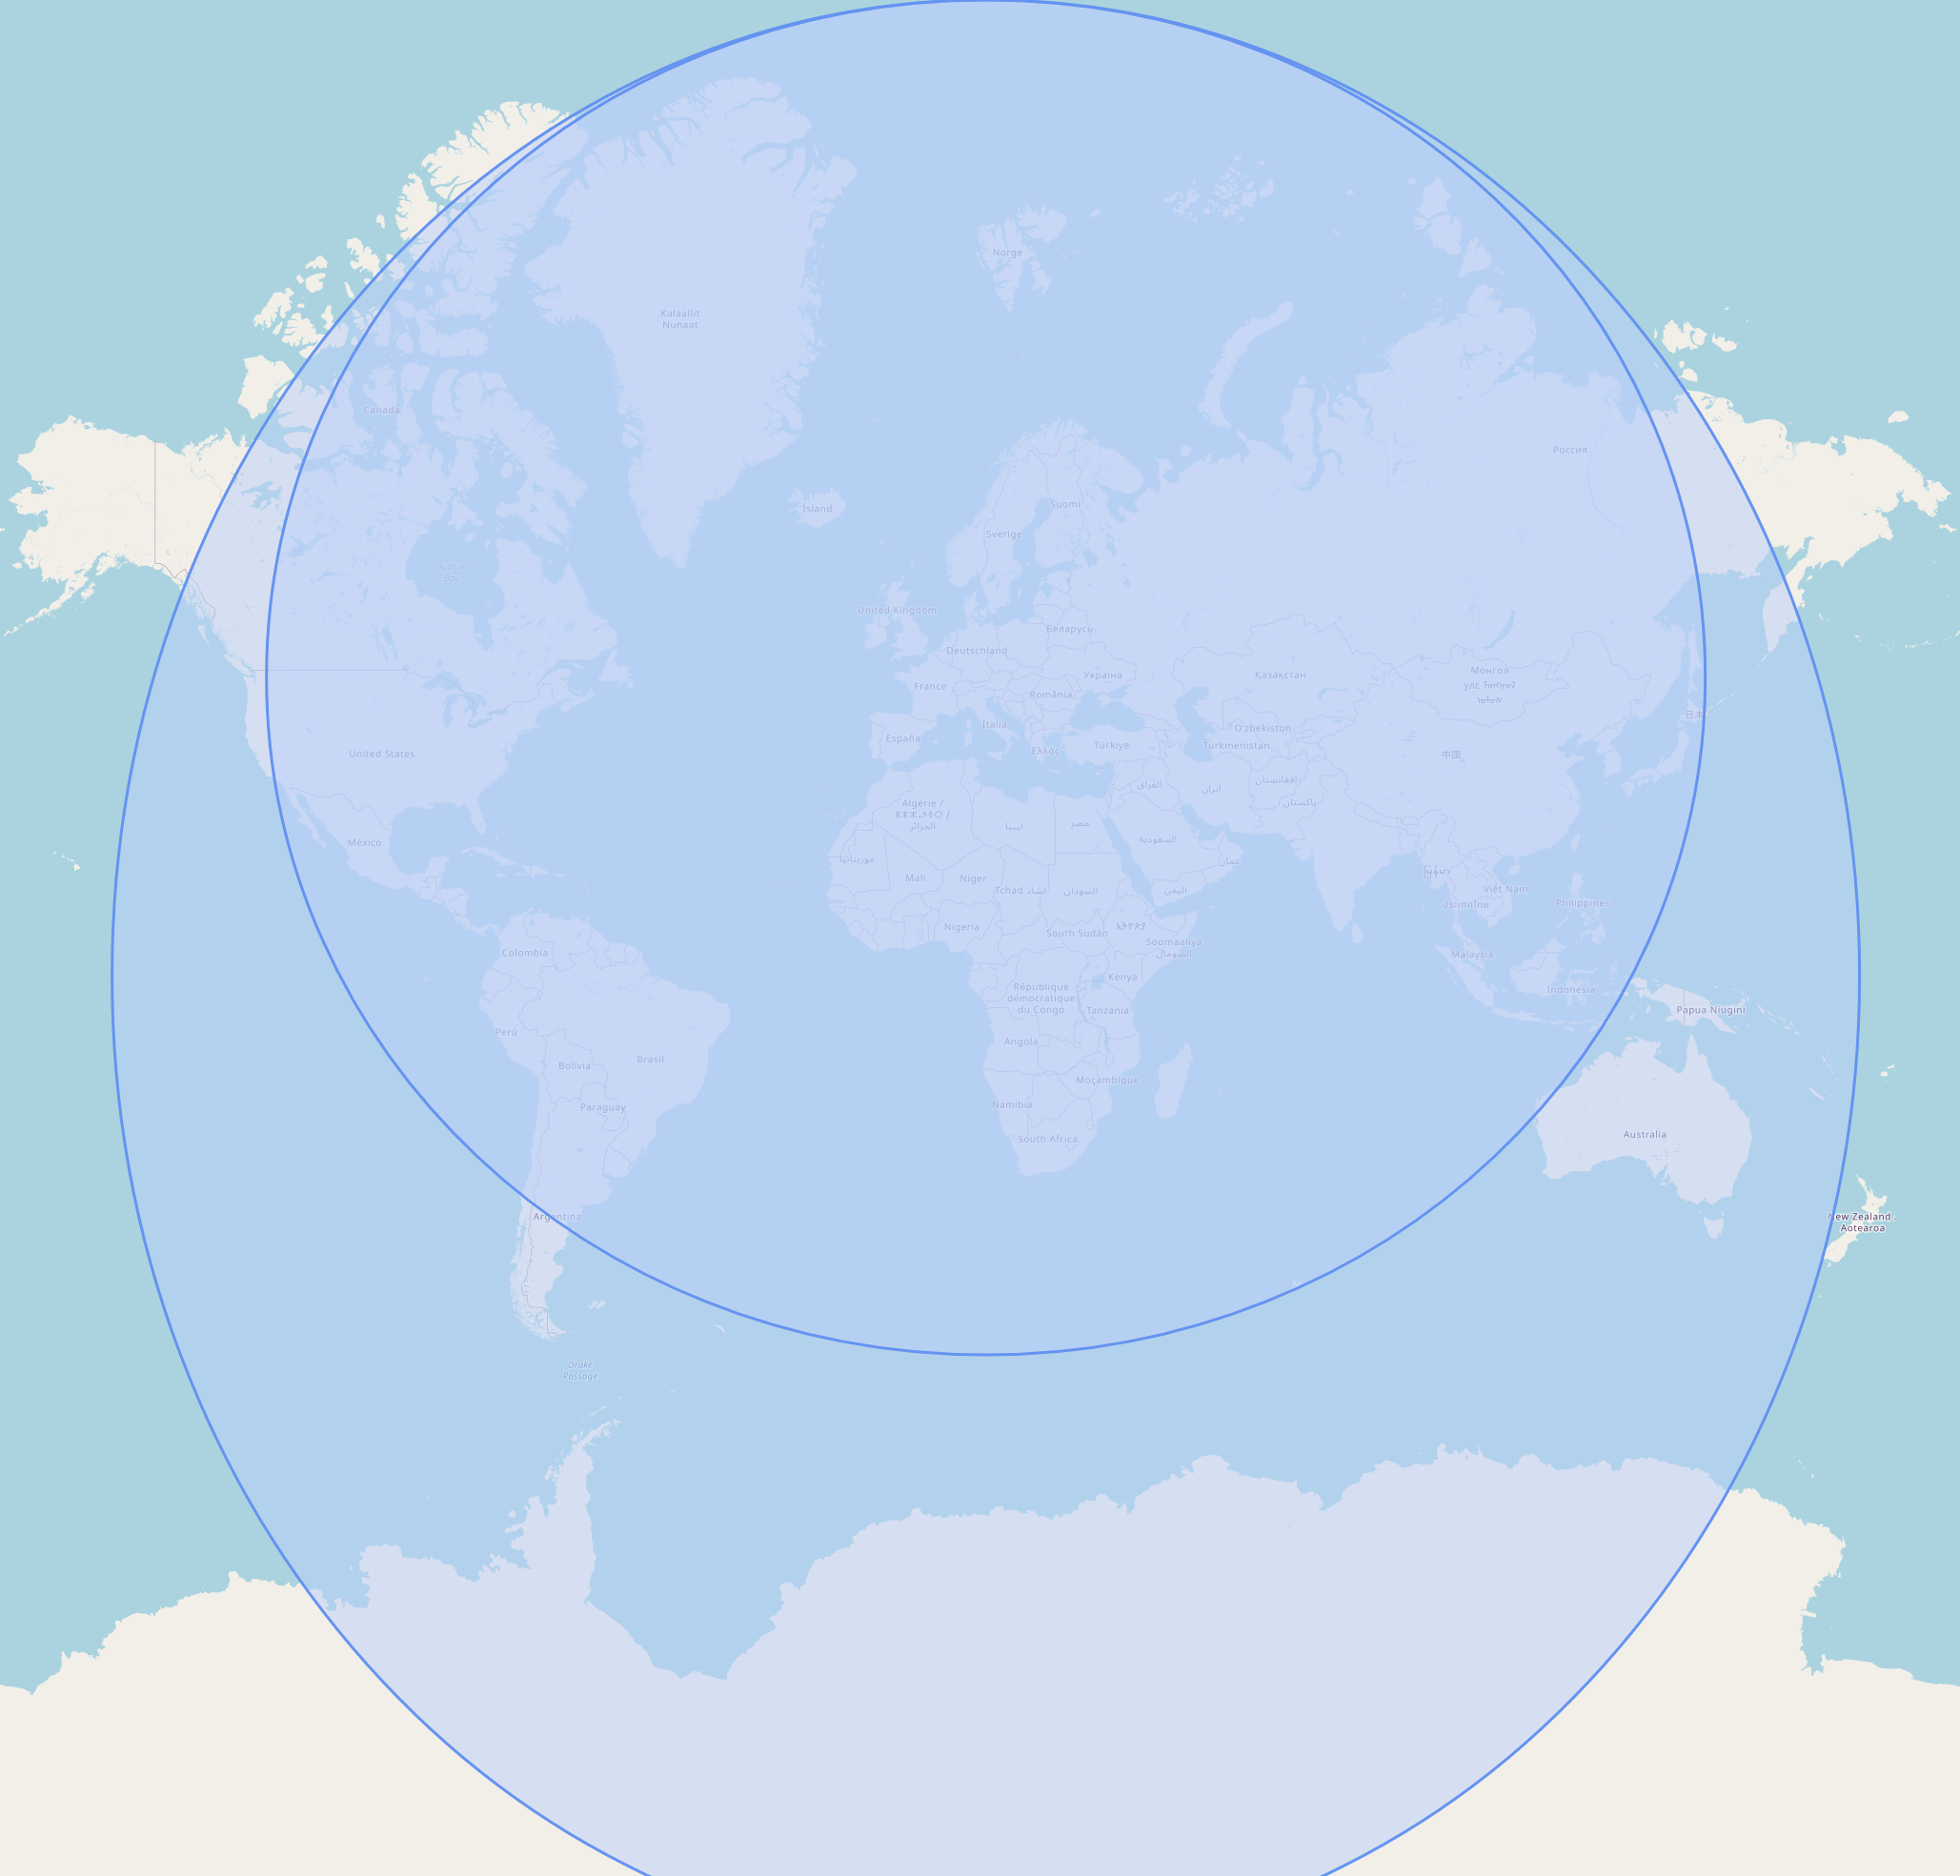
\includegraphics[width=0.95\textwidth]{Sources/Plots_and_Pictures/OSM_radius.png}
    \caption{Global coverage at 11000 km and 15000 km. Notice that the circles are concentric,
    but the maximum range exceeds the global scale of the map, which shifts the largest circle}
    \label{Global_Coverage}
\end{figure}
\clearpage

The aircraft could easily cover a continuous intercontinental flight between many of the major cities around the globe.\\ 
The following dark theme maps are from \textit{GNOME Maps} \autocite{Gnome_maps}. 

\begin{figure}[h!]
    \phantomsection
    \centering
    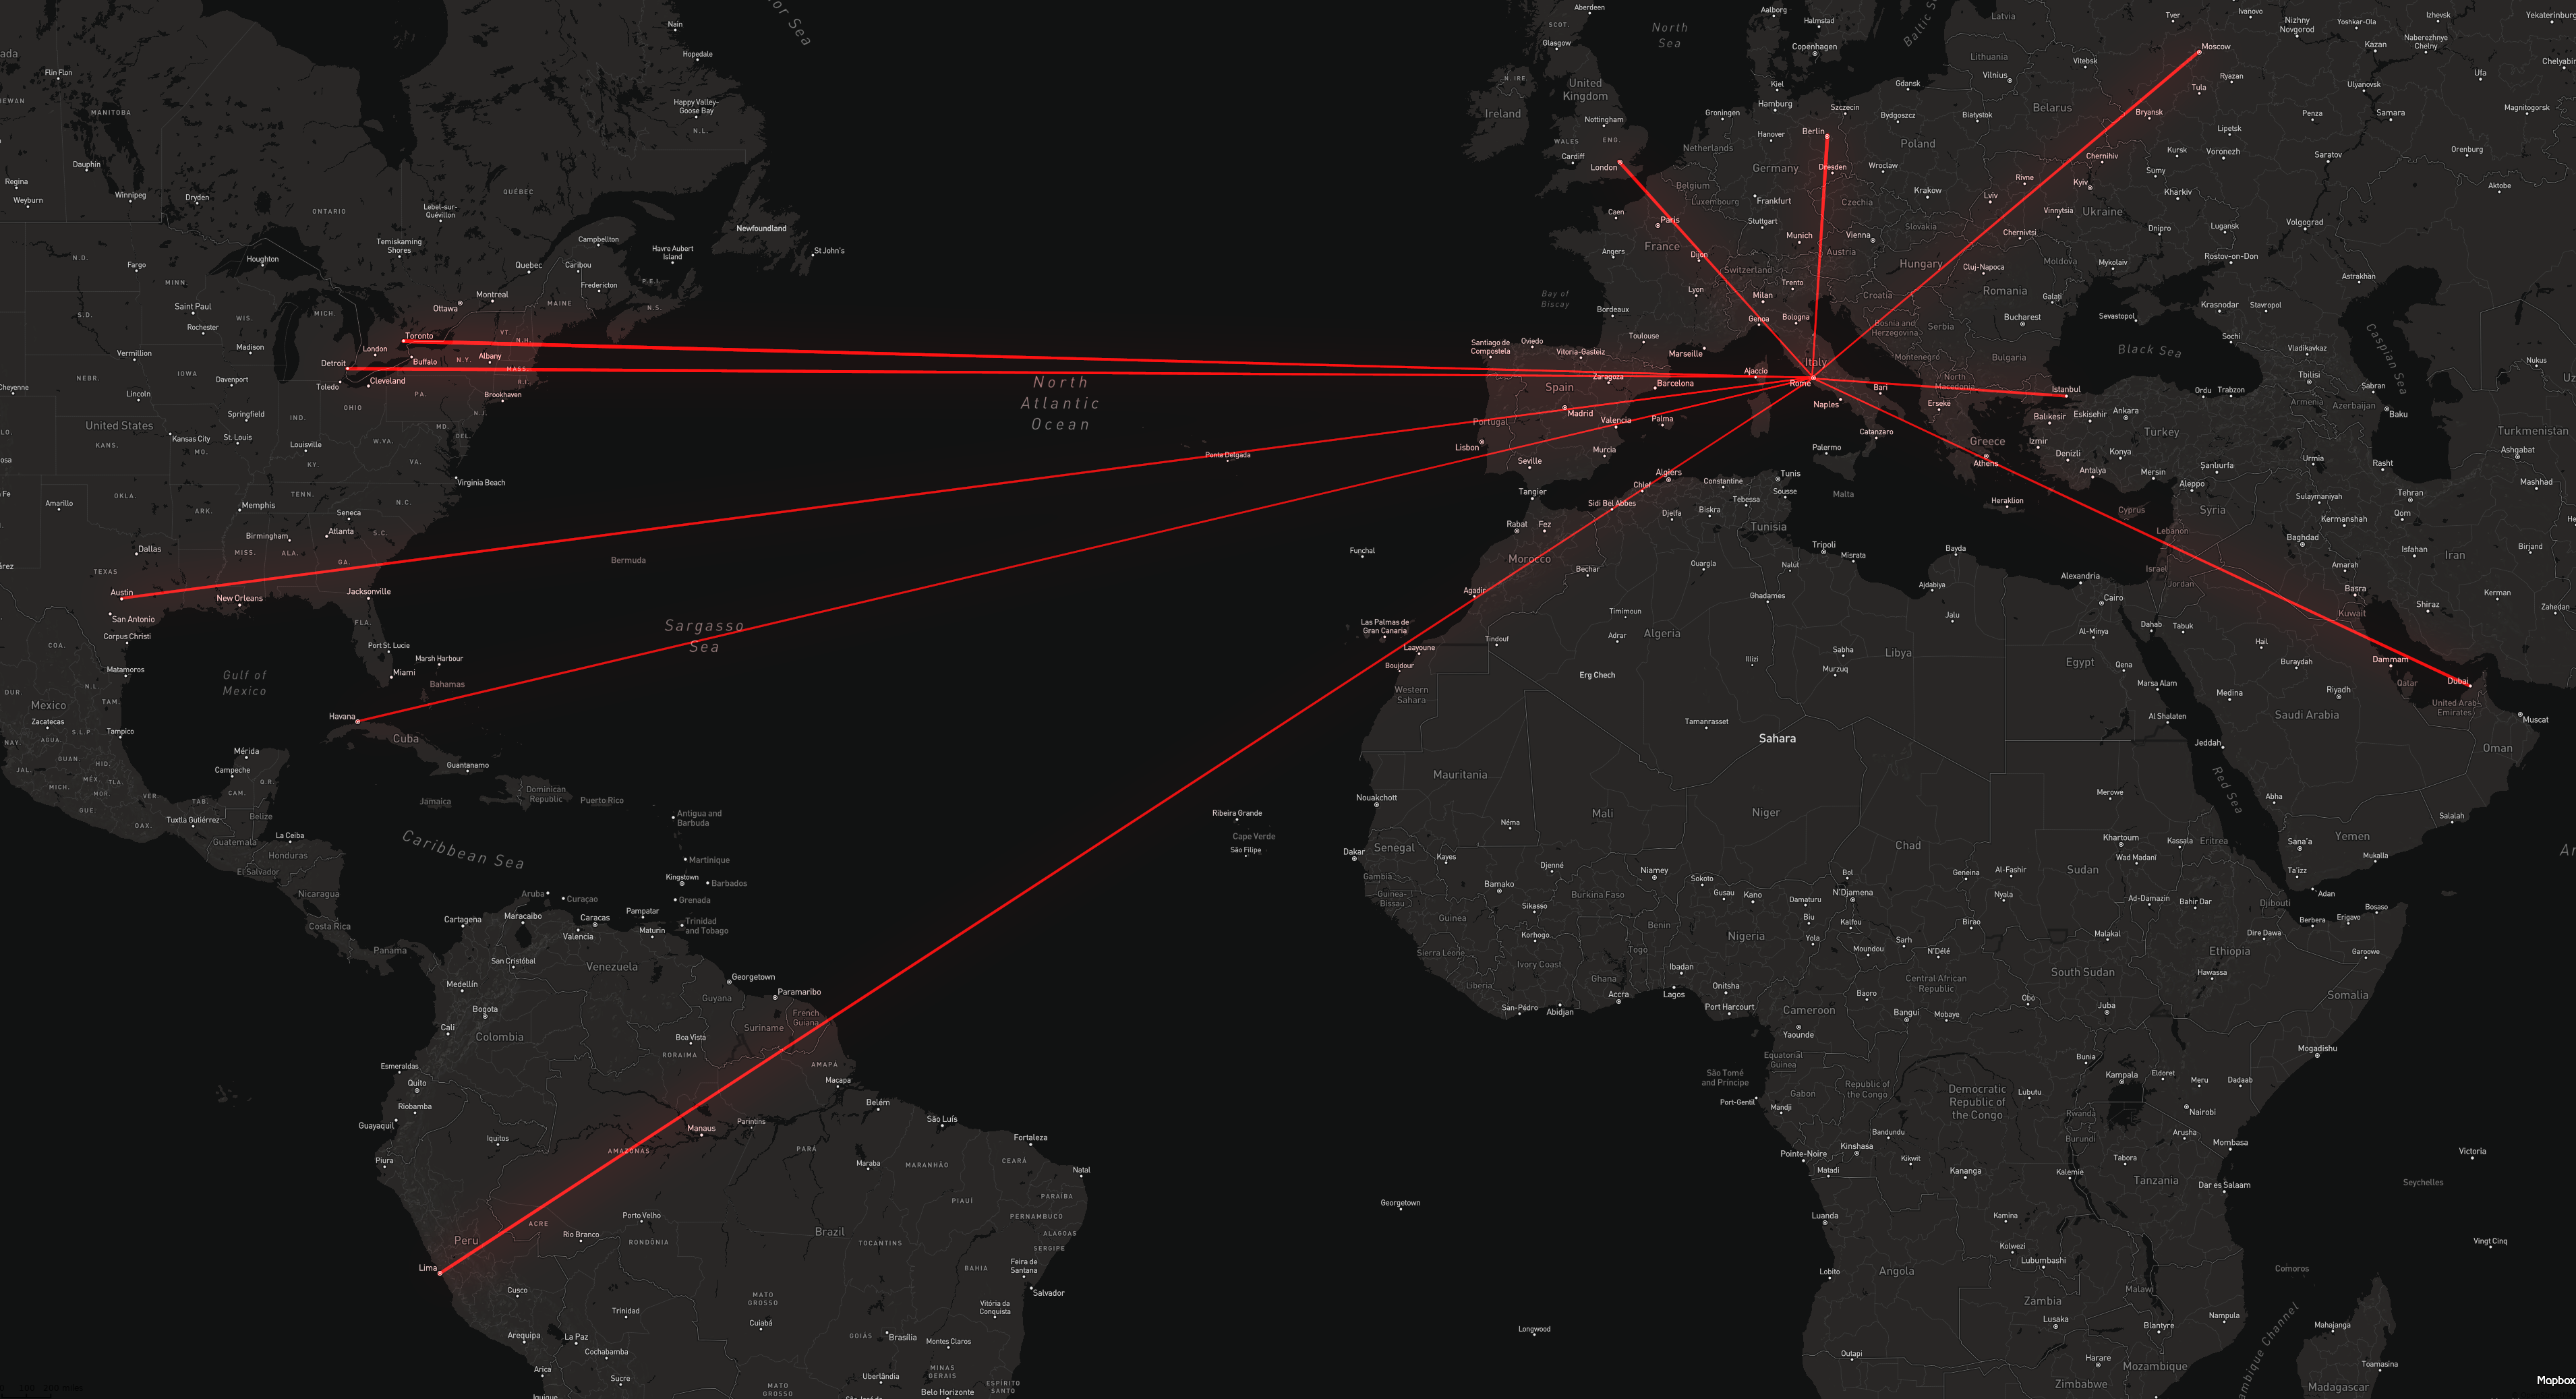
\includegraphics[width=\textwidth]{Sources/Plots_and_Pictures/worldwide_routes.png}
    \caption{Many major cities linked with Rome}
    \label{worldwide_maps}
\end{figure}
For instance, it could easily link Rome to Los Angeles (10189.91 km), even at full payload
and still have fuel left.
\begin{figure}[h!]
    \phantomsection
    \centering
    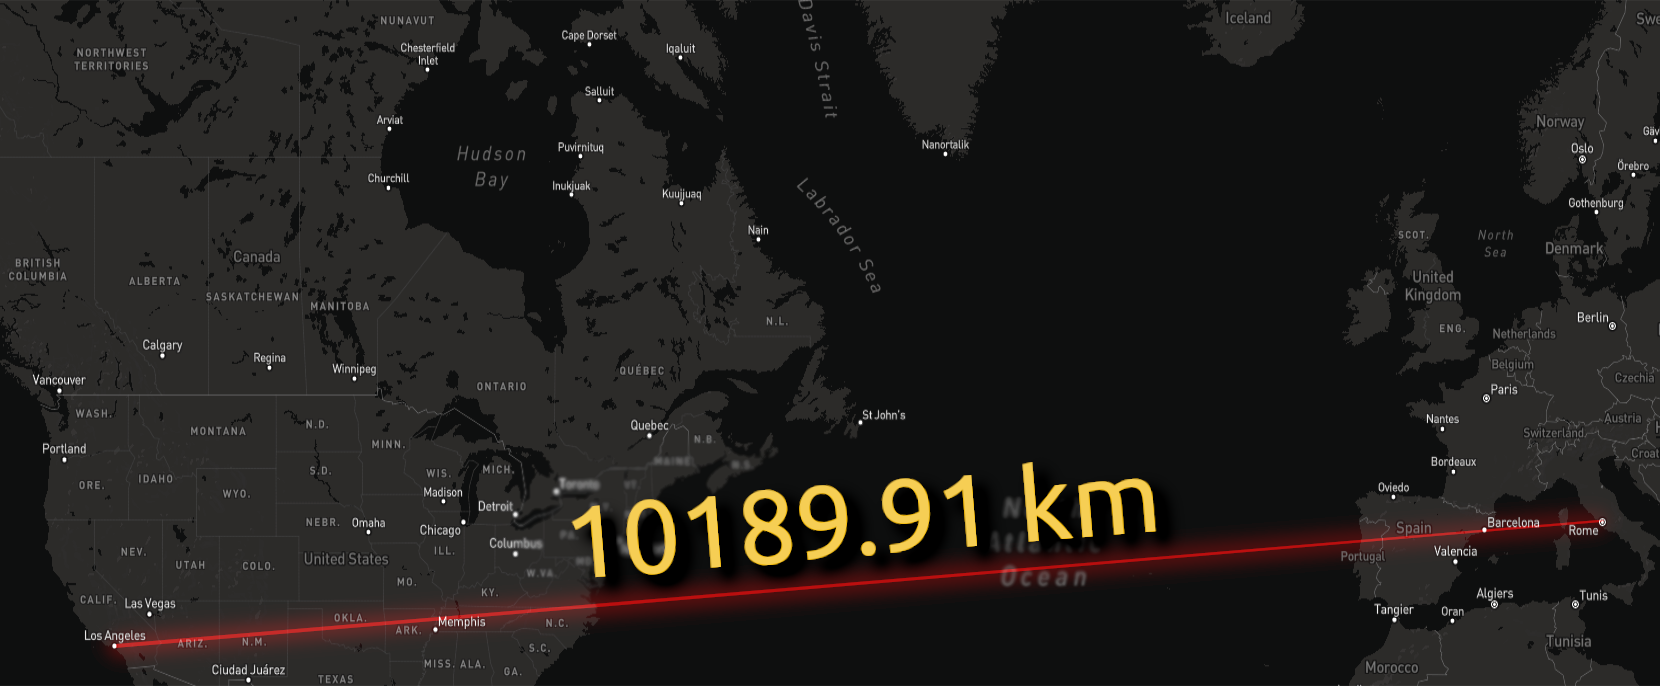
\includegraphics[width=\textwidth]{Sources/Plots_and_Pictures/rome_LA.png}
    \caption{Rome - Los Angeles}
    \label{rome_LA}
\end{figure}

\clearpage

A few more examples: 

\begin{itemize}
    \item Rome - Las Vegas (9834.85 km, full payload)
    \item Rome - Toronto (7081.70 km, full payload)
    \item Rome - Vancouver (8992.46 km, full payload)
    \item Rome - Mexico City (10240.82 km, full payload)
    \item Rome - Lima (10861.53 km, full payload)
    \item Rome - Beijing (8122.88 km, full payload)
    \item Rome - Tokyo (9857.88 km, full payload)
    \item Rome - Cape Town (8452.22 km, full payload)
    \item Rome - Buenos Aires (11150.43 km)
\end{itemize}


\clearpage



However, an interesting way of exploiting its range, would be a hypothetical route among multiple city-pairs, with no
refuel between the trips and immediate departure. \\ \\ 
Using \textit{DistanceFromTo} \autocite{City_Distance_Calculator}, another tool built with Open Street Map and Leaflet, an example of
a route starting and coming all the way back to Rome has been estimated to be around 13899.78 km. \\ 
The route has then been drawn on the map below, using \textit{GIMP} \autocite{GIMP}. \\ 

\begin{figure}[h!]
    \phantomsection
    \centering
    \includegraphics[width=\textwidth]{Sources/Plots_and_Pictures/route.png}
    \caption{Example of a long range no-refuel route}
    \label{Global_Coverage}
\end{figure}
\clearpage


\pagebreak 

\subsection{Assignment 2.4\label{Assignment_2.4}}
\textbf{Assignment:} Build the Matching Chart for your case study and define
 Wing Surface and Engine Thrust \\ \\ \\ 

 \subsubsection{Stall Velocity\label{stall_velocity}}

 Stall velocity is calculated by dividing
 the approach velocity by 1.3 (as described by regulations). \\ 
 The approach velocity is guessed by comparison with similar aicrafts, as suggested by Daniel P. Raymer \autocite{Raymer_Daniel}.\\ 
 A value of 145 knots has been chosen, as it's in between the A350-900 and A350-1000.\\ 

 \subsubsection{Key cruise parameters\label{cruise_parameters}}

 Once the necessary fuel for the 11000 km range has been consumed, the landing mass is around 214000 kg,
 which is in line with the statistical population range of $[205000, 236000] \ kg$.\\ 
 As suggested by Daniel P. Raymer \autocite{Raymer_Daniel}, an air density equivalent
 to that of sea level is assumed for all the calculations. \\ 
 The author also suggests a maximum lift coefficient between 2.2 and 3.2, thus a value
 of 2.8 has been chosen.\\ 
 Given the density, the stall velocity and the maximum lift coefficient, the function \autocite{Airbus_replacement_repo}
 \begin{verbatim}
    wing_load_distribution.m
 \end{verbatim}
calculates the $\frac{W}{S}$  $[\frac{kg}{m^2}]$, which is going to be a recurring variable later on.
With a result of $575.60 \ \frac{kg}{m^2}$ the value is in the established range. 

Using the design \textit{MTOW}, the estimated wing surface is $489.97 \ m^2$. \\ 

It is crucial that the wing load's numerator is converted to \textit{N}, in order to get a dimensionless
Thrust to Weight ratio.\\ 
The ratio is calculated for the maximum cruise speed, by the function 
\begin{verbatim}
    thrust_weight_max_speed.m
\end{verbatim}



\clearpage

The ratio is then calculated by taking the \textit{TOP} (Take Off Parameter) into account, by the function 
\begin{verbatim}
    thrust_weight_TOP.m
\end{verbatim}
which takes the lift coefficient at takeoff as an input.\\ 

The \textit{TOP} is estimated to be around $230 \ \frac{lbs}{ft^2}$, with a \textit{ground roll distance}
of 3000 ft (888 m) and a 1.7 times higher \textit{over 50 feet distance}.\\ 
As suggested by Jan Roskam \autocite{Roskam}, the lift coefficient at takeoff is the maximum lift coefficient
divided by a factor of 1.21. \\ 

Another equation for the Thrust to Weight ratio is based on the \textit{ROC} (Rate Of Climb), 
and has been implemented into the function

\begin{verbatim}
    thrust_weight_ROC.m
\end{verbatim}

Finally, knowing the $\frac{W}{S}$, the design \textit{MTOW} and the \textit{Thrust to Weight Ratio} at takeoff, 
the function 
\begin{verbatim}
    thrust_design.m
\end{verbatim}

calculates the design \textit{Required Thrust}, which amounts to 691849 N.

\clearpage

\subsubsection{Design Point and Matching Chart\label{Matching_chart}}

The design point has been chosen in a way that minimizes wing surface, which in turns
increases the necessary thrust.

However, since the available thrust of the chosen engine is substantially higher than initially
planned, the tradeoff is acceptable.

\begin{figure}[h!]
    \phantomsection
    \centering
    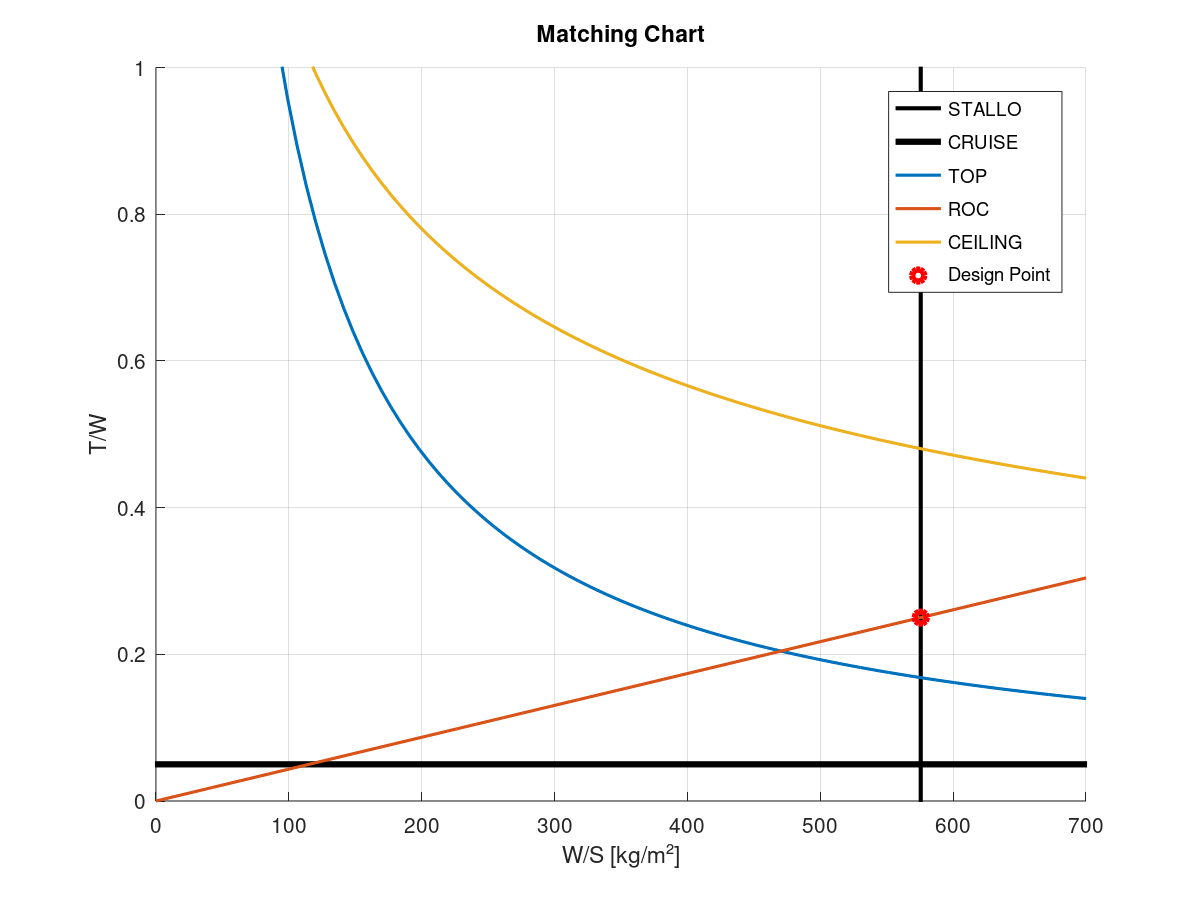
\includegraphics[width=\textwidth]{Sources/Plots_and_Pictures/Matching_chart.png}
    \caption{Matching Chart}
    \label{matching_chart}
\end{figure}
\clearpage

\section{Assignment 3\label{Assignment_3}}

\subsection{Assignment 3.1\label{Assignment_3.1}}

\textbf{\textit{Assignment:}} Following the procedure suggested in the previous charts,
and on the basis of the parameters estimated in previous assignments,
define your own wing airfoil. \\ \\ \\ 

Initially, the profile that was opted for was the \textit{GOE 682}, with a 30 degrees sweep angle, 
as suggested by Daniel P. Raymer \autocite{Raymer_Daniel}.

However, that allowed for a suboptimal \textit{set angle} of 1 degree, thus leading to another alternative.

After some research on \textit{Airfoiltools} \autocite{Airfoiltools}, the final choice was in favor
of the \textit{NACA1412}, which provides a maximum lift coefficient of 1.51, as well as an ideal lift coefficient
for a \textit{set angle} of 3.5 degrees.

The maximum lift coefficient should be more than enough and actually a good safety margin 
for a stall scenario.

In addition to this, the presence of \textit{HLD} (High Lift Devices) has been assumed, with 
a 0.9 and 0.4 lift coefficient contribution for flaps and slats, respectively (as suggested by Mohammad H. Sadraey \autocite{Sadraey_Mohammad}).\\ 

\begin{figure}[h!]
    \phantomsection
    \centering
    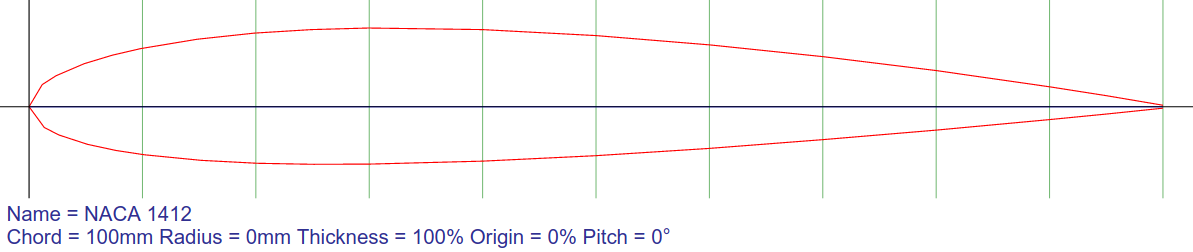
\includegraphics[width=\textwidth]{Sources/Plots_and_Pictures/NACA1412.png}
    \caption{NACA1412}
    \label{NACA1412}
\end{figure}
\clearpage

The function \autocite{Airbus_replacement_repo} 
\begin{verbatim}
    max_gross_lift_coeff_calculator.m
\end{verbatim}
calculates the \textit{gross lift coefficient}.\\

Given an \textit{Aspect Ratio} of 9, the wing surface and its \textit{sweep angles} of $ \{29, 18 \} \ deg$,
the function 
\begin{verbatim}
    wing_profile_plotter.m
\end{verbatim}
plots the wing profile, as seen from an above POV, while also returning a \textit{Taper Ratio} of 0.31915.\\ 

\begin{figure}[h!]
    \phantomsection
    \centering
    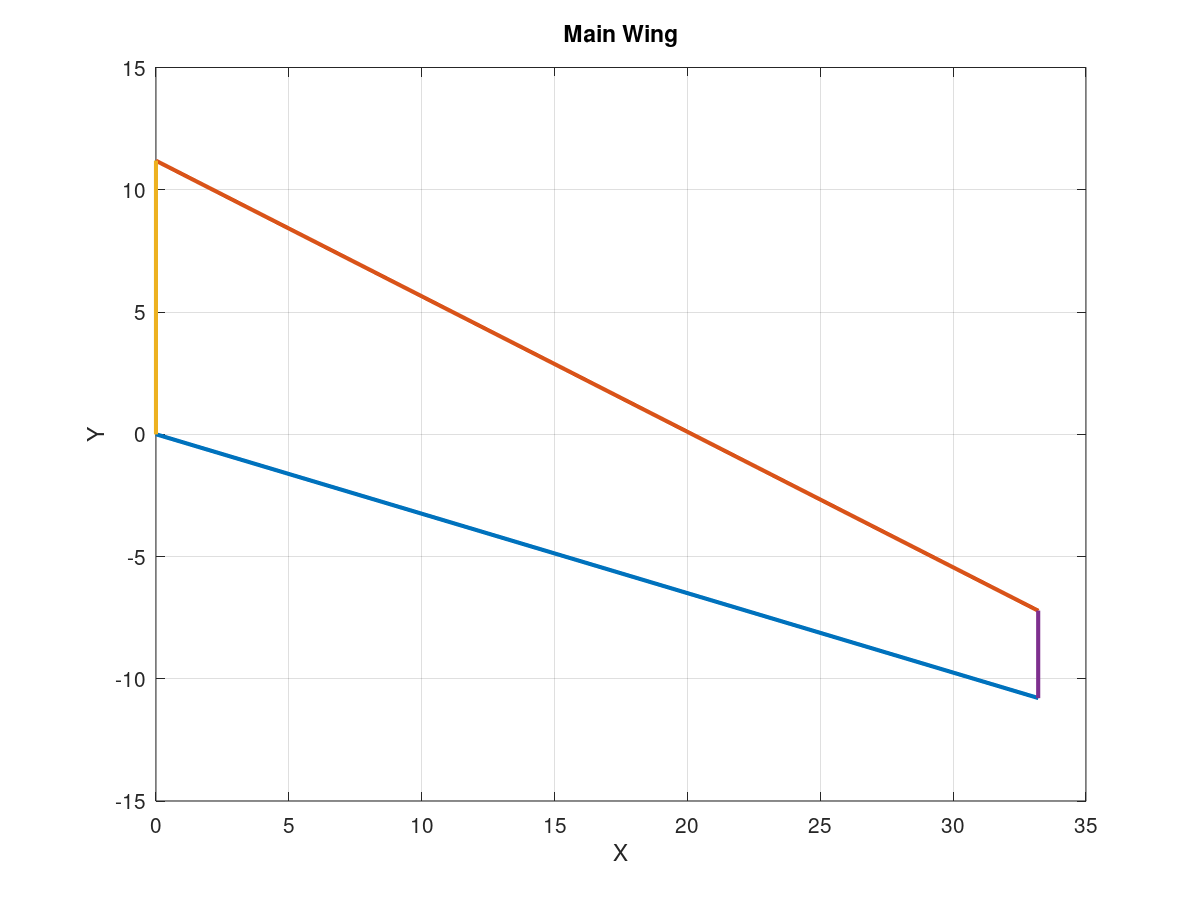
\includegraphics[width=\textwidth]{Sources/Plots_and_Pictures/Main_Wing.png}
    \caption{Main Wing}
    \label{Main_wing}
\end{figure}

The function is also used later on to plot the tail wings, as it requires the type of wing to plot as one of its inputs.\\
\clearpage

As the highest \textit{Reynolds} given by \textit{Airfoiltools} is $10^6$, a comparative check on the 
actual \textit{Reynolds} should be run, in order to see whether the values given by the website are 
accurate or not.\\ 
For this purpose, the needed \textit{MAC} (Mean Aerodynamic Center) is calculated by the 
function \autocite{Airbus_replacement_repo}
\begin{verbatim}
    mean_aerodynamic_center.m
\end{verbatim}
which is based on an approximation given by Daniel P. Raymer \autocite{Raymer_Daniel}. \\ 

Then, the current \textit{Reynolds} is compared to the maximum value given by the website, by the function

\begin{verbatim}
    reynolds_check.m
\end{verbatim}

As hoped, the values are not too different, thus validating the rest of the data.\\ 
\clearpage

\subsection{Assignment 3.2\label{Assignment_3.2}}

\textbf{\textit{Assignment:}} Once the airfoil has been selected, look for reference materials
showing aerodynamic coefficients trends. 
Are they in line with your expectations (and requirements)? 



\clearpage

\subsection{Assignment 3.3\label{Assignment_3.3}}

\textbf{\textit{Assignment:}} Once the wing airfoil is selected, please, 
try to identify the main parameters for a 3D wing. 
\clearpage 
\subsection{Assignment 3.4\label{Assignment_3.4}}

\textbf{\textit{Assignment:}} 2D and 3D CAD Modelling 

\clearpage 

\section{Assignment 4\label{Assignment_4}}

\subsection{Assignment 4.1\label{Assignment_4.1}}

\textbf{\textit{Assignment:}} Design your fuselage following the suggested methodology\\ \\ \\ 

The general procedure was implemented following Muhammad H. Sadraey's workflow and suggested values \autocite{Sadraey_Mohammad},
and by taking the \textit{EASA CS-25.807, Amendment 3} \autocite{EASA_CS25} regulations into account.\\ 

The configuration that was opted for is the following: 
\begin{itemize}
    \item \textit{Business} (26 seats)
        \begin{itemize}
            \item 1, 2, 1
            \begin{itemize}
                \item $\left ( 70, 104, 75 \right ) \ cm$ \\ (Corridor Width, Room between seats, Seat Width)
            \end{itemize}
        \end{itemize}
    \item \textit{First Class} (48 seats)
        \begin{itemize}
            \item 2, 2, 2
            \begin{itemize}
                \item $\left ( 60, 92, 60 \right ) \ cm$ \\ (Corridor Width, Room between seats, Seat Width)
            \end{itemize}
        \end{itemize}
    \item \textit{Economy Class} (315 seats)
        \begin{itemize}
            \item 3, 3, 3
            \begin{itemize}
                \item $\left ( 50, 72, 46 \right ) \ cm$ \\ (Corridor Width, Room between seats, Seat Width)
            \end{itemize}
        \end{itemize}
\end{itemize}
\clearpage

As suggested by the author, the nose length is calculated with a slightly different
formula for each class and the tail zone is 1 m longer than the nose. 

The doors dimensions are strictly tied to the regulations and both the number and type have been 
chosen accordingly, as visible in the CAD model. 
Furthermore, a thickness of 102 mm has been added to the fuselage, as established by regulations. 

Four \textit{1X1 m} toilet modules have been installed and considered in the calculations, this time according to Daniel P. Raymer \autocite{Raymer_Daniel}.\\ 

The function \autocite{Airbus_replacement_repo}
\begin{verbatim}
    passenger_mass_calculator.m
\end{verbatim}

estimates and returns a vector with the mass of passengers for each available class, based on the number of seats and
the average human mass, as well as an extra mass budget for each seat, which varies with the class itself.\\ 

The resulting mass is $\left \{ 3328,  \  6144, \  37485 \right \} \ kg$ for Business, First Class and Economy respectively. \\ 

The function 
\begin{verbatim}
    fuselage_size_calculator.m
\end{verbatim}

accepts as inputs each class' geometry vectors, as well as a vector with the number of seats for each class, 
and returns a dimensions vector for each class, as well as the total fuselage length. \\ 

The results are the following:
\begin{itemize}
    \item \textit{Business Dimensions} (W X L)
        \subitem  $\left \{4.4000, \ 6.7600 \right \} \ m$
    \item \textit{First Class Dimensions} (W X L)
        \subitem  $\left \{4.8000, \ 7.3600 \right \} \ m$
    \item \textit{Economy Dimensions} (W X L)
        \subitem  $\left \{5.1400, \ 25.2000 \right \} \ m$
    \item \textit{Total Fuselage Length}
        \subitem  67.304 m
\end{itemize}

\clearpage


\subsection{Assignment 4.2\label{Assignment_4.2}}

\textbf{\textit{Assignment:}} Create your Fuselage in Solidworks 
and validate your fuselage concept

\clearpage

\section{Assignment 5\label{Assignment_5}}

\subsection{Assignment 5.1\label{Assignment_5.1}}

\textbf{\textit{Assignment:}} Select and briefly justify the most appropriate
 tail configuration for your case study \\ \\ \\ 

The conventional or inverted T-shape configuration was an immediate choice, as it's a simple, widely
used and yet effective design. 

In addition to this, as suggested by Mohammad H. Sadraey \autocite{Sadraey_Mohammad}, this traditional design is more appropriate
for inexperienced aircraft designers. \\ 

This configuration includes one horizontal tail mounted on the
aft fuselage and one vertical tail on top of the aft fuselage.

While they both deal with various stability requirements, the former handles longitudinal trim, 
the latter handles directional trim. \\ 


\begin{figure}[h!]
    \phantomsection
    \centering
    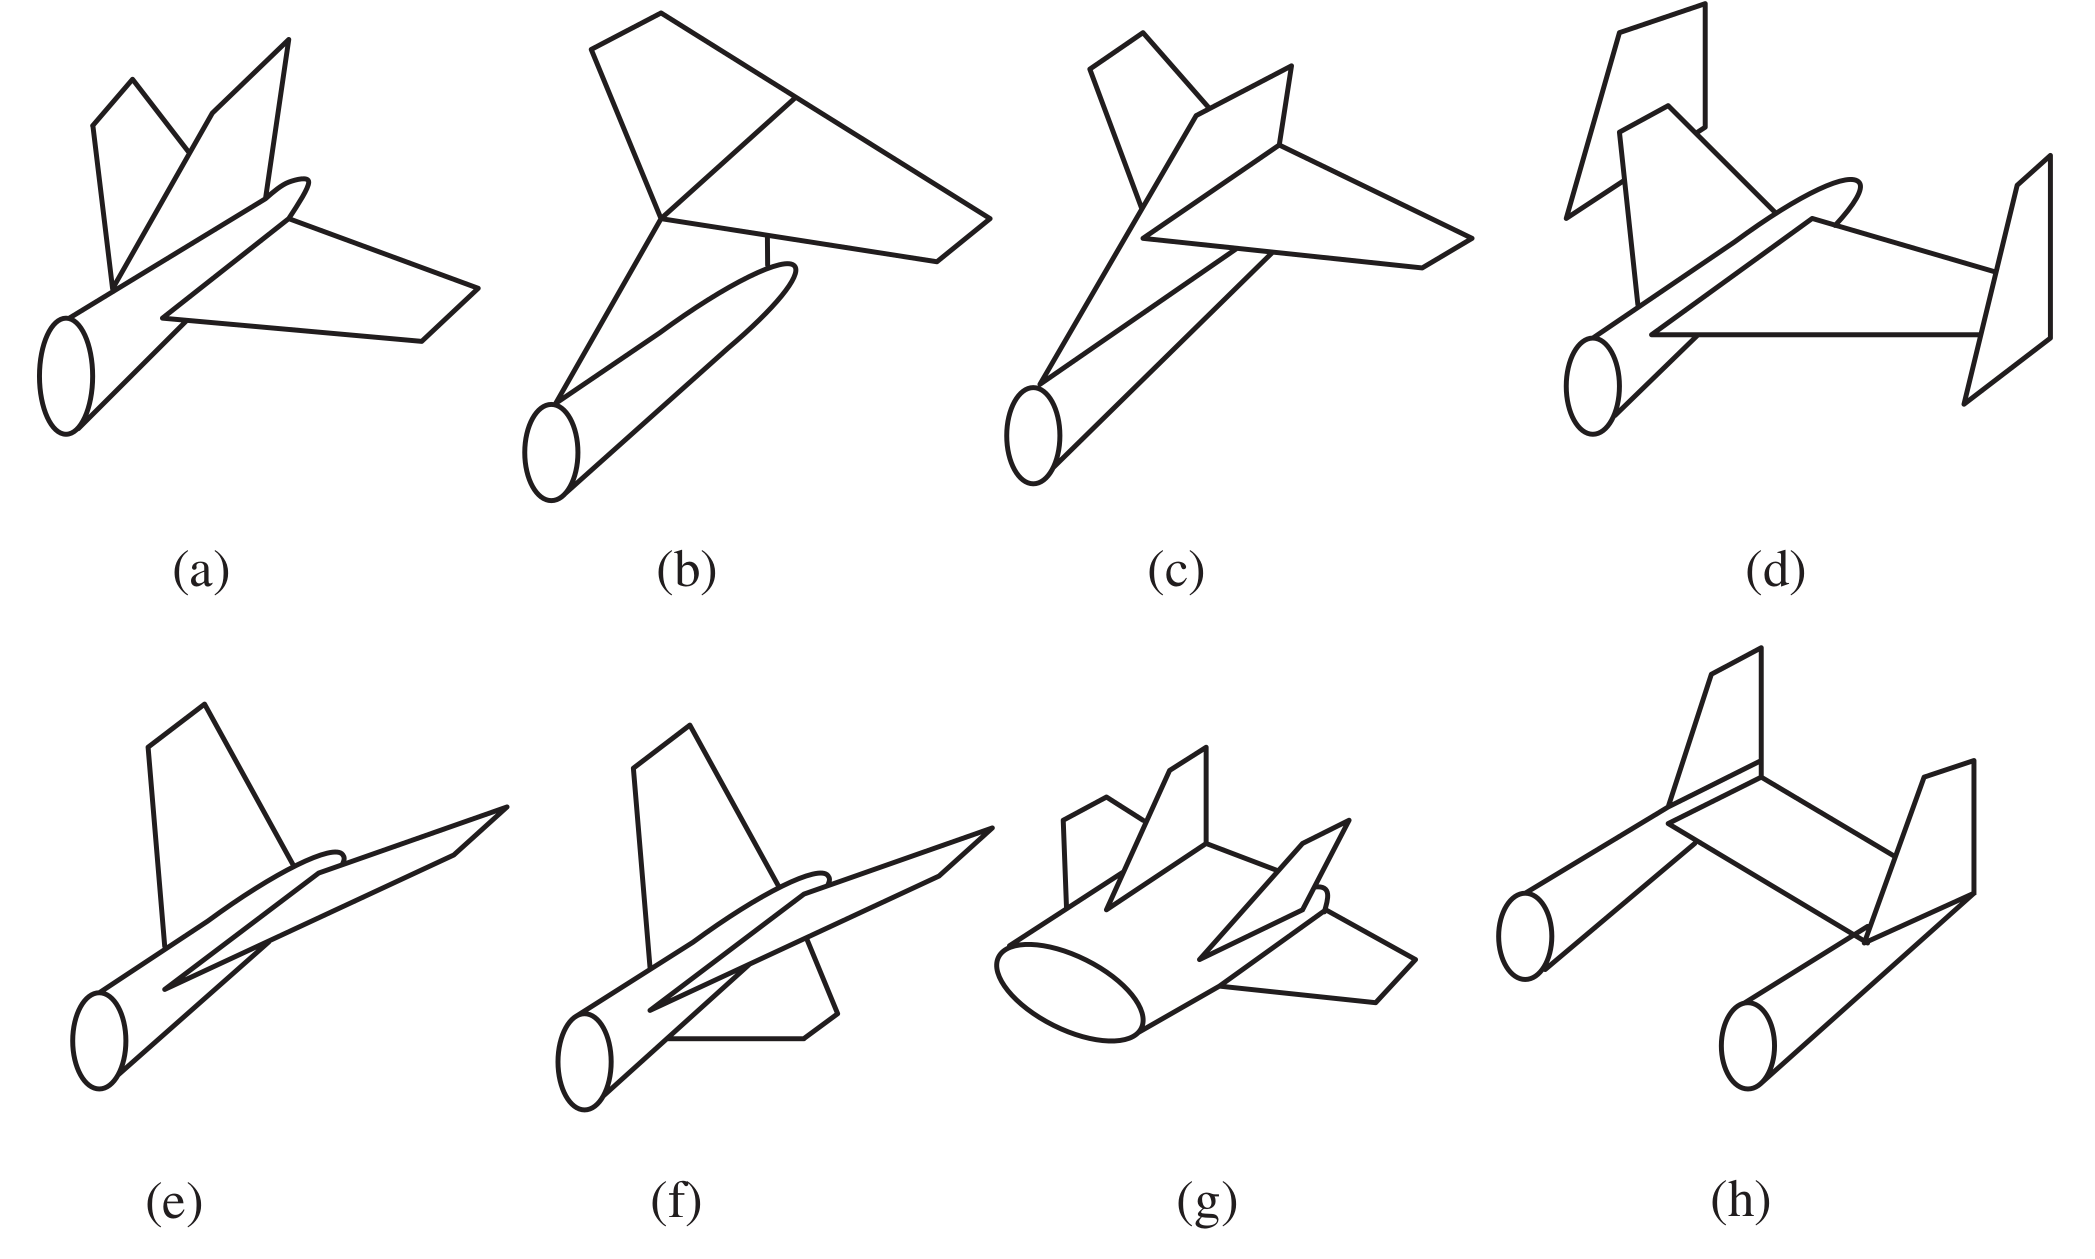
\includegraphics[width=\textwidth]{Sources/Plots_and_Pictures/tail_config.png}
    \caption{Several tail configurations: \textbf{(a) Conventional}; (b) T-tail; (c) Cruciform; (d) H-tail;
    (e)V-tail; (f) Y-tail; (g) Twin vertical tail; (h) Boom mounted \autocite{Sadraey_Mohammad}}
    \label{tail_config}
\end{figure}

\clearpage

\subsection{Assignment 5.2\label{Assignment_5.2}}

\textbf{\textit{Assignment:}} Follow the procedure reported in these charts
 and size your horizontal tail plane. \\ \\ \\ 

As once again suggested by Mohammad H. Sadraey \autocite{Sadraey_Mohammad}, a \textit{NACA0012} profile 
has been chosen, as it's symmetric and not excessively thick. \\ 

\begin{figure}[h!]
    \phantomsection
    \centering
    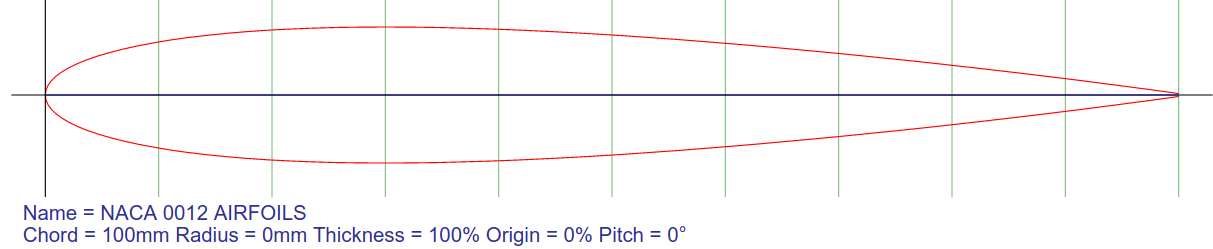
\includegraphics[width=\textwidth]{Sources/Plots_and_Pictures/NACA0012.png}
    \caption{NACA0012 \autocite{Airfoiltools}}
    \label{NACA0012}
\end{figure}


The author supplies a table with typical volume coefficients for both the horizontal and the vertical tail.
The reference values are, of course, those for \textit{Jet Transport} aircrafts.\\ 

\begin{table}[h!]
    \centering
    \resizebox{\textwidth}{!}{%
    \begin{tabular}{@{}lcc@{}}
    \rowcolor[HTML]{9B9B9B} 
    \textbf{Aircraft} &
      \multicolumn{1}{l}{\cellcolor[HTML]{9B9B9B}\textbf{Horizontal tail Volume Coefficient}} &
      \multicolumn{1}{l}{\cellcolor[HTML]{9B9B9B}\textbf{Vertical Tail Volume Coefficient}} \\
    \rowcolor[HTML]{FFFFFF} 
    Glider and motor glider      & 0.6 & 0.03 \\
    \rowcolor[HTML]{EFEFEF} 
    GA twin prop-driven engine   & 0.5 & 0.04 \\
    \rowcolor[HTML]{FFFFFF} 
    GA single prop-driven engine & 0.7 & 0.04 \\
    \rowcolor[HTML]{EFEFEF} 
    GA twin prop-driven engine   & 0.8 & 0.07 \\
    \rowcolor[HTML]{FFFFFF} 
    GA with canard               & 0.6 & 0.05 \\
    \rowcolor[HTML]{EFEFEF} 
    Agricultural                 & 0.5 & 0.04 \\
    \rowcolor[HTML]{FFFFFF} 
    Twin turboprop               & 0.9 & 0.08 \\
    \rowcolor[HTML]{EFEFEF} 
    Jet trainer                  & 0.7 & 0.06 \\
    \rowcolor[HTML]{FFFFFF} 
    Fighter aircraft             & 0.4 & 0.07 \\
    \rowcolor[HTML]{EFEFEF} 
    Fighter (with canard)        & 0.1 & 0.06 \\
    \rowcolor[HTML]{FFFFFF} 
    Bomber/military transport    & 1   & 0.08 \\
    \rowcolor[HTML]{EFEFEF} 
    Jet transport                & 1.1 & 0.09
    \end{tabular}%
    }
    \caption{Typical values for horizontal and vertical tail volume coefficients \autocite{Sadraey_Mohammad}}
    \label{tab:volume_coefficients}
    \end{table}
\clearpage


 The function \autocite{Airbus_replacement_repo}

\begin{verbatim}
    tail_surface_calculator.m
\end{verbatim}

has been implemented: it evaluates the optimal distance and use it to return the wing surface, following the author's workflow. 

The same function is later used to calculate the vertical wing's surface, as it takes the tail wing type as one of the inputs.

The result was a $94.435 \ m^2$ surface. \\ 

The Taper Ratio is recommended to be between 0.4 and 0.7, thus a value of 0.6 has been chosen.

This allows for a wing span of 20 m, which is comparable to the 18 m of the A350. \\ 

As for the set angle, the function \autocite{Airbus_replacement_repo}

\begin{verbatim}
    set_angle_calculator.m
\end{verbatim}

returns its value, after taking some typical wing angles as an input. The assumption made was that of horizontal
cruise, at constant velocity. \\ 

The function 

\begin{verbatim}
    horizontal_tail_aero_coefficients_calculator.m
\end{verbatim}

calculates a pair of useful aerodynamic coefficients for the tail wing, returning the following values:

\begin{itemize}
    \item ${C_{M0}^{\ (wing body)} = -0.014731} $
    \item ${C_{L}^{\ (tail)}} = 0.069604$
\end{itemize}


\clearpage

The sweep angles are the same as the main wing, the \textit{MAC} (Mean Aerodynamic Center) is calculated
and the wing is plotted with the same functions implemented for the main wing [\ref{Assignment_3.1}].

\begin{figure}[h!]
    \phantomsection
    \centering
    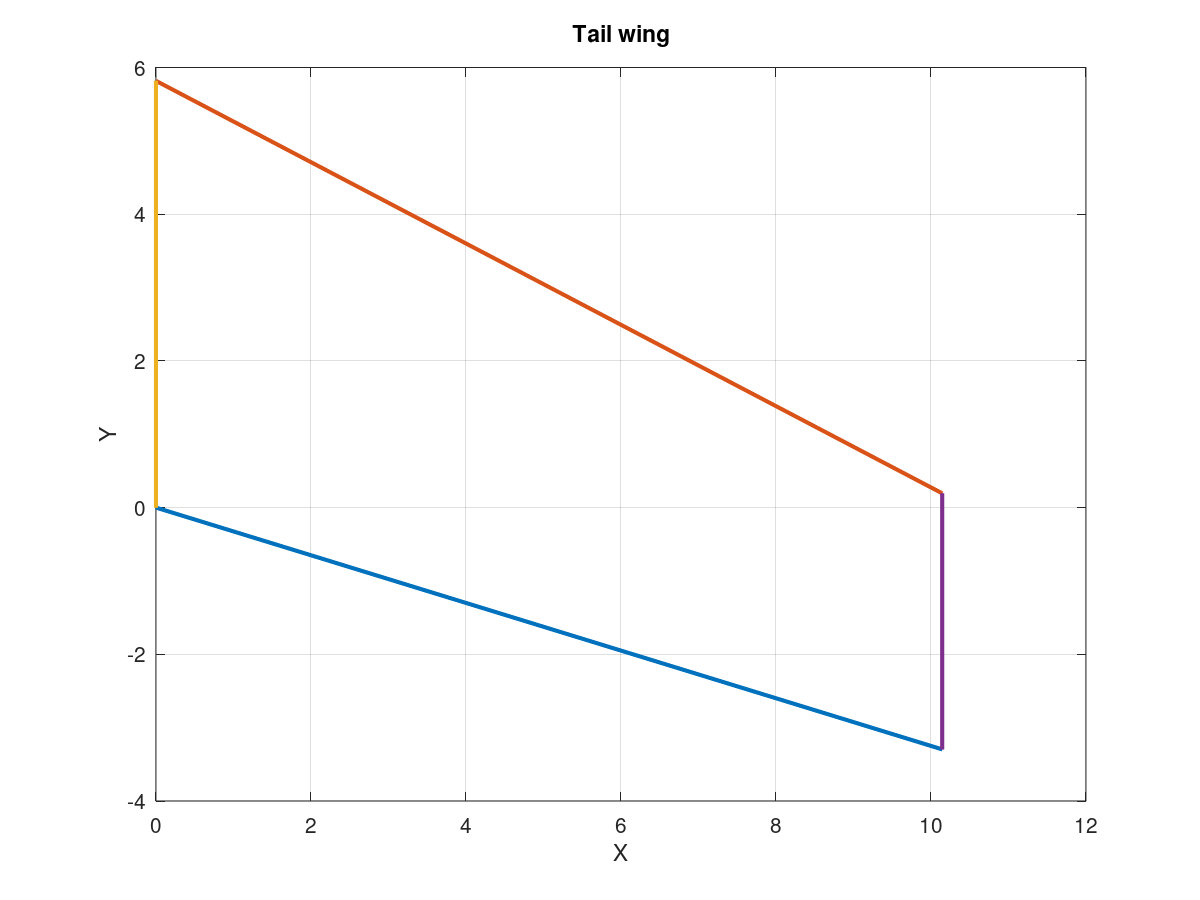
\includegraphics[width=\textwidth]{Sources/Plots_and_Pictures/Tail_Wing.png}
    \caption{Horizontal Tail Wing}
    \label{Horizontal_tail}
\end{figure}


\clearpage

\subsection{Assignment 5.3\label{Assignment_5.3}}

\textbf{\textit{Assignment:}} Follow the procedure reported in these charts
 and size your vertical tail plane. \\ \\ \\ 

The procedure for the vertical tail wing is very similar to the horizontal one and, as suggested by 
Mohammad H. Sadraey \autocite{Sadraey_Mohammad}, the optimal distance between the \textit{MAC} and the tail
is the same as the horizontal one.\\ 

The \textit{NACA0012} \autocite{Airfoiltools} has been chosen again, mostly for its symmetry and relatively
low thickness.\\ 

\begin{figure}[h!]
    \phantomsection
    \centering
    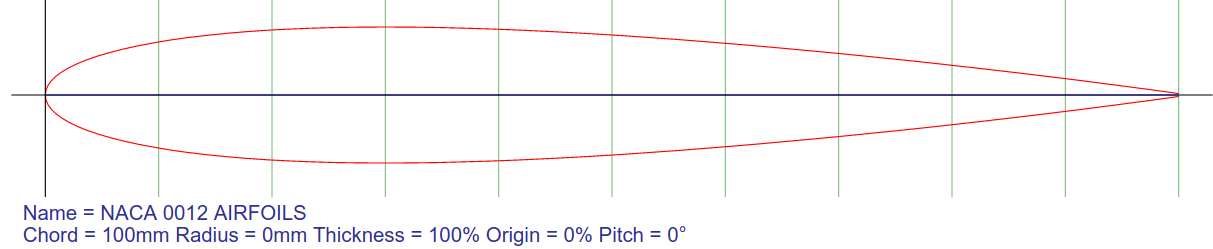
\includegraphics[width=\textwidth]{Sources/Plots_and_Pictures/NACA0012.png}
    \caption{NACA0012 \autocite{Airfoiltools}}
    \label{NACA0012_vert}
\end{figure}

The set angle is null, as the aircraft is equipped with twin engines that provide a symmetrical and 
equally distributed thrust, unlike single front fan aircrafts, where a set angle might be used
in order to compensate the net reaction torque generated by the single engine. 

The \textit{Aspect Ratio} and the \textit{Taper Ratio} have been kept equal to those of the Airbus A350-900 \autocite{Airbus_A350-900}.

As suggested by Mohammad H. Sadraey \autocite{Sadraey_Mohammad}, the highest \textit{Sweep Angle} has been
chosen to be $35^{\circ}$, which is in line with the statistical population as well. 

Using trigonometry, the other angle is geometrically calculated, with an estimated value of $10.767^{\circ}$. 
\clearpage 

With the workflow seen in section \ref{Assignment_5.2}, a wing surface of $210.51 \ m^2$ has been calculated
and the vertical tail wing has been plotted.

\begin{figure}[h!]
    \phantomsection
    \centering
    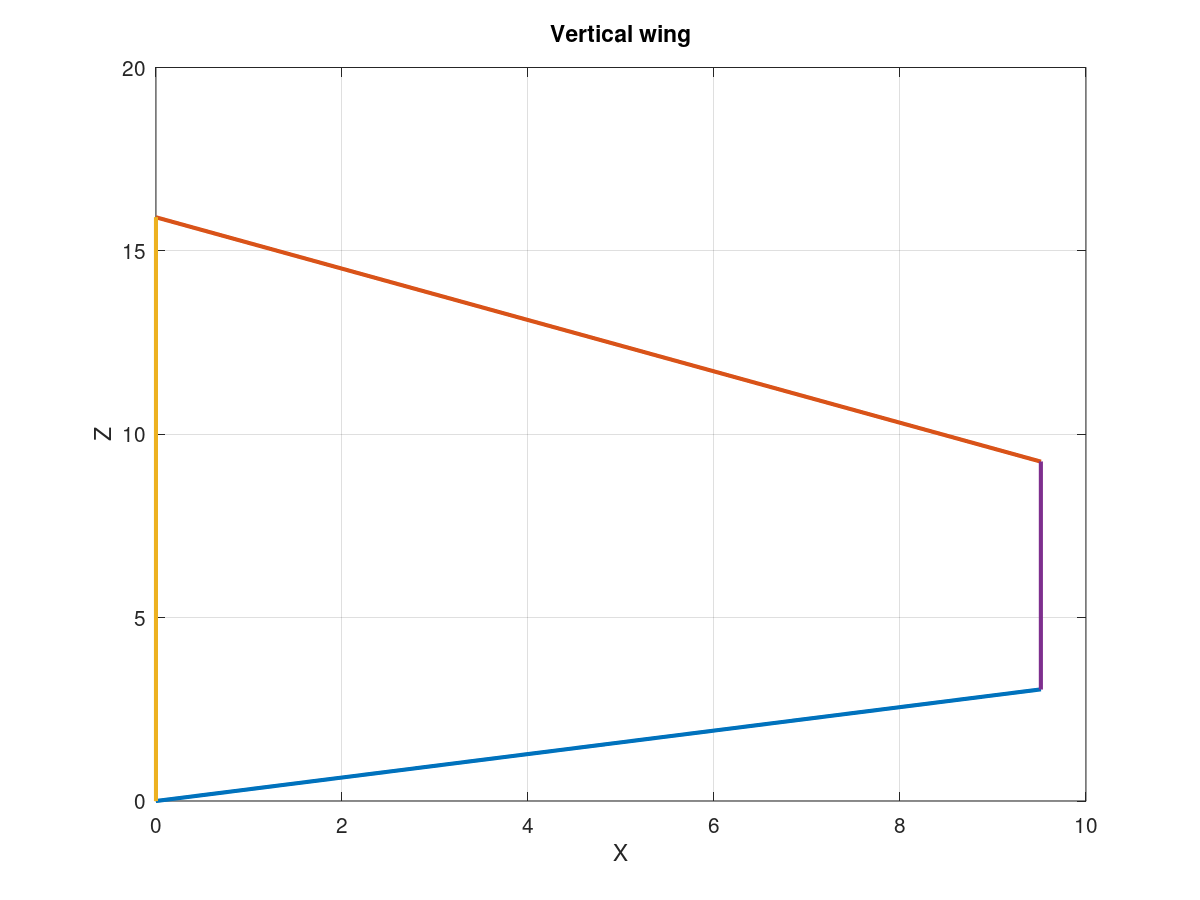
\includegraphics[width=\textwidth]{Sources/Plots_and_Pictures/Vertical_Wing.png}
    \caption{NACA0012}
    \label{vertical_wing}
\end{figure}


\clearpage

\subsection{Assignment 5.4\label{Assignment_5.4}}

\textbf{\textit{Assignment:}} Develop a CAD model 
of the sized aircraft tail \\ \\ \\ 

\clearpage

\section{Assignment 6\label{Assignment_6}}

\subsection{Assignment 6.1\label{Assignment_6.1}}

\textbf{\textit{Assignment:}} Apply the lifting-line theory to the 3D wing model already defined
and if necessary, indicate possible improvements to be performed to guarantee sufficient lift generation \\ \\ \\ 

Wing lift analysis is very sensitive to \textit{Taper Ratio} variations, whose value is typically between 
0.3 and 0.4 in literature, as this range allows for the minimum \textit{Lift-induced Drag}, thus leading to 
an optimal lift distribution. \\ 

The function \autocite{Airbus_replacement_repo}

\begin{verbatim}
    lifting_line_plotter.m
\end{verbatim}

is an implementation of the \textit{Lifting line theory} and is based upon a script provided by Mohammad H. Sadraey \autocite{Sadraey_Mohammad}. 

It returns the wing's \textit{Lift coefficient}, which resulted to be 0.39334 and plots the lift coefficient as a function of the semi-wingspan.

The function also runs a check to verify whether the contribution of the wing to the total lift is at least $85 \%$ (the test was passed). \\ 

This theory is based upon very strong assumptions and oversimplifications, which make it suitable for cruise
conditions only. 

The wing aerodynamic performance derived from this model can't therefore be used for more critical scenarios, like
specific maneuvers, proximity to stall conditions or landing and takeoff. \\ 

\begin{figure}[h!]
    \phantomsection
    \centering
    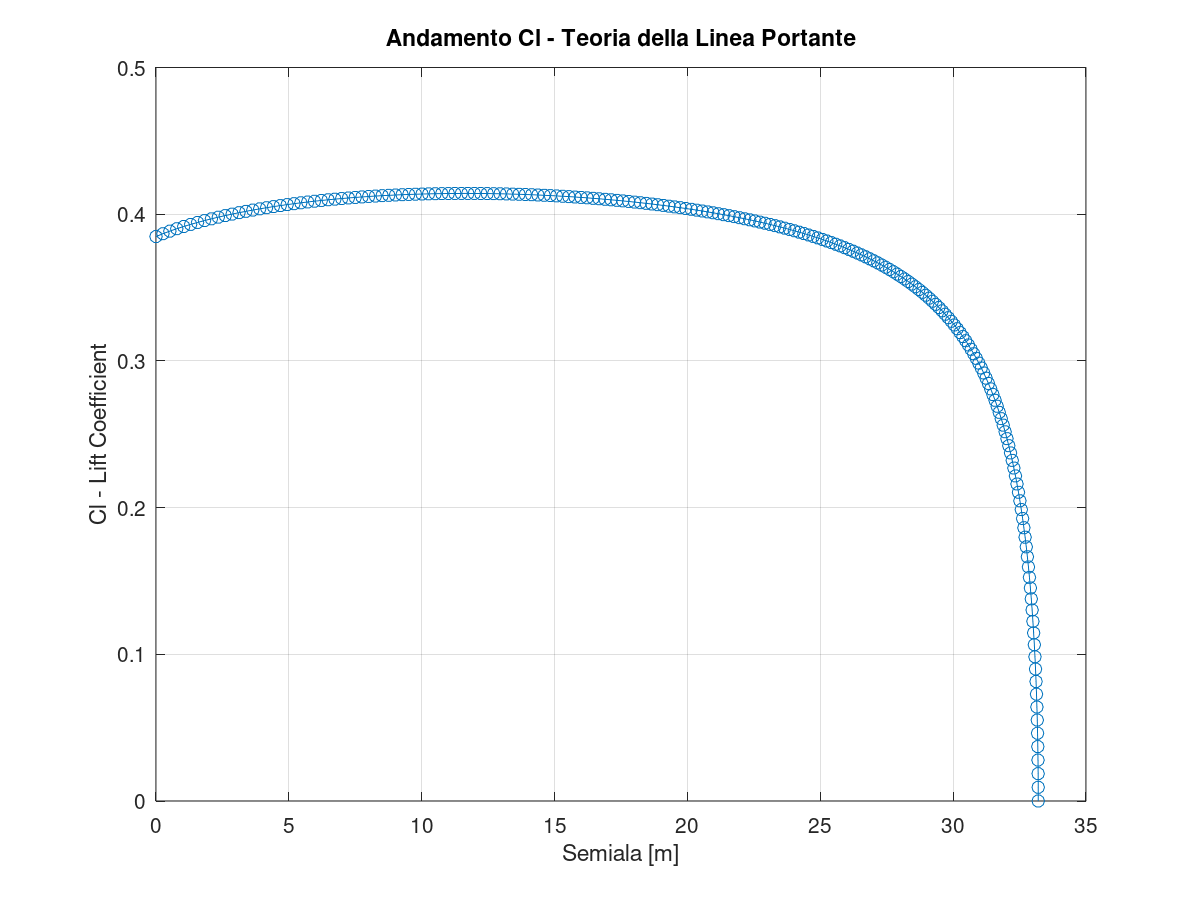
\includegraphics[width=0.55\textwidth]{Sources/Plots_and_Pictures/Linea_Portante.png}
    \caption{Lifting line: The result is close to an elliptical distribution, which would be the ideal case}
    \label{lifting_line}
\end{figure}


\clearpage


\subsection{Assignment 6.2\label{Assignment_6.2}}

\textbf{\textit{Assignment:}} Apply one of the two suggested methods and define your selected engine \\ \\ \\ 

As seen in section \ref{cruise_parameters}, the total \textit{Required Thrust} amounts to 691849 N, which
translates to 345.924 kN per engine, in a twin engine design.\\ 

Given its widespread use for this class of aircraft and its efficiency, the engine research focused on a 
\textit{Turbofan}, rather than a \textit{Turbojet} or \textit{Turboprop}. 

The chosen approach was that of looking for an already existing engine in the market, as there's plenty of available
options that would satisfy the requirements. \\ 

A great source of public domain information on all kinds of aeronautic engines is the well known \textit{ICAO}
database on engines' emissions \autocite{ICAO_engine_database}.

The database provides an exhaustive list of all sorts of engines, as well as accurate and up to date info on their market availability
status and, of course, their key parameters, like thrust and many others. \\ 

Having taken a good look at the database and having seen the typical options for aircrafts of the same family,
the most appealing options were \textit{Rolls Royce} and \textit{General Electric} engines. \\ 

After some more in depth research, the final choice was in favor of the \textit{General Electric GE90-94B}. 

An essential design point is that the available thrust is higher than the required one. 
This engine meets this vital requirement, while also being an overall reliable and high performance device. 


\clearpage

\begin{figure}[h!]
    \phantomsection
    \centering
    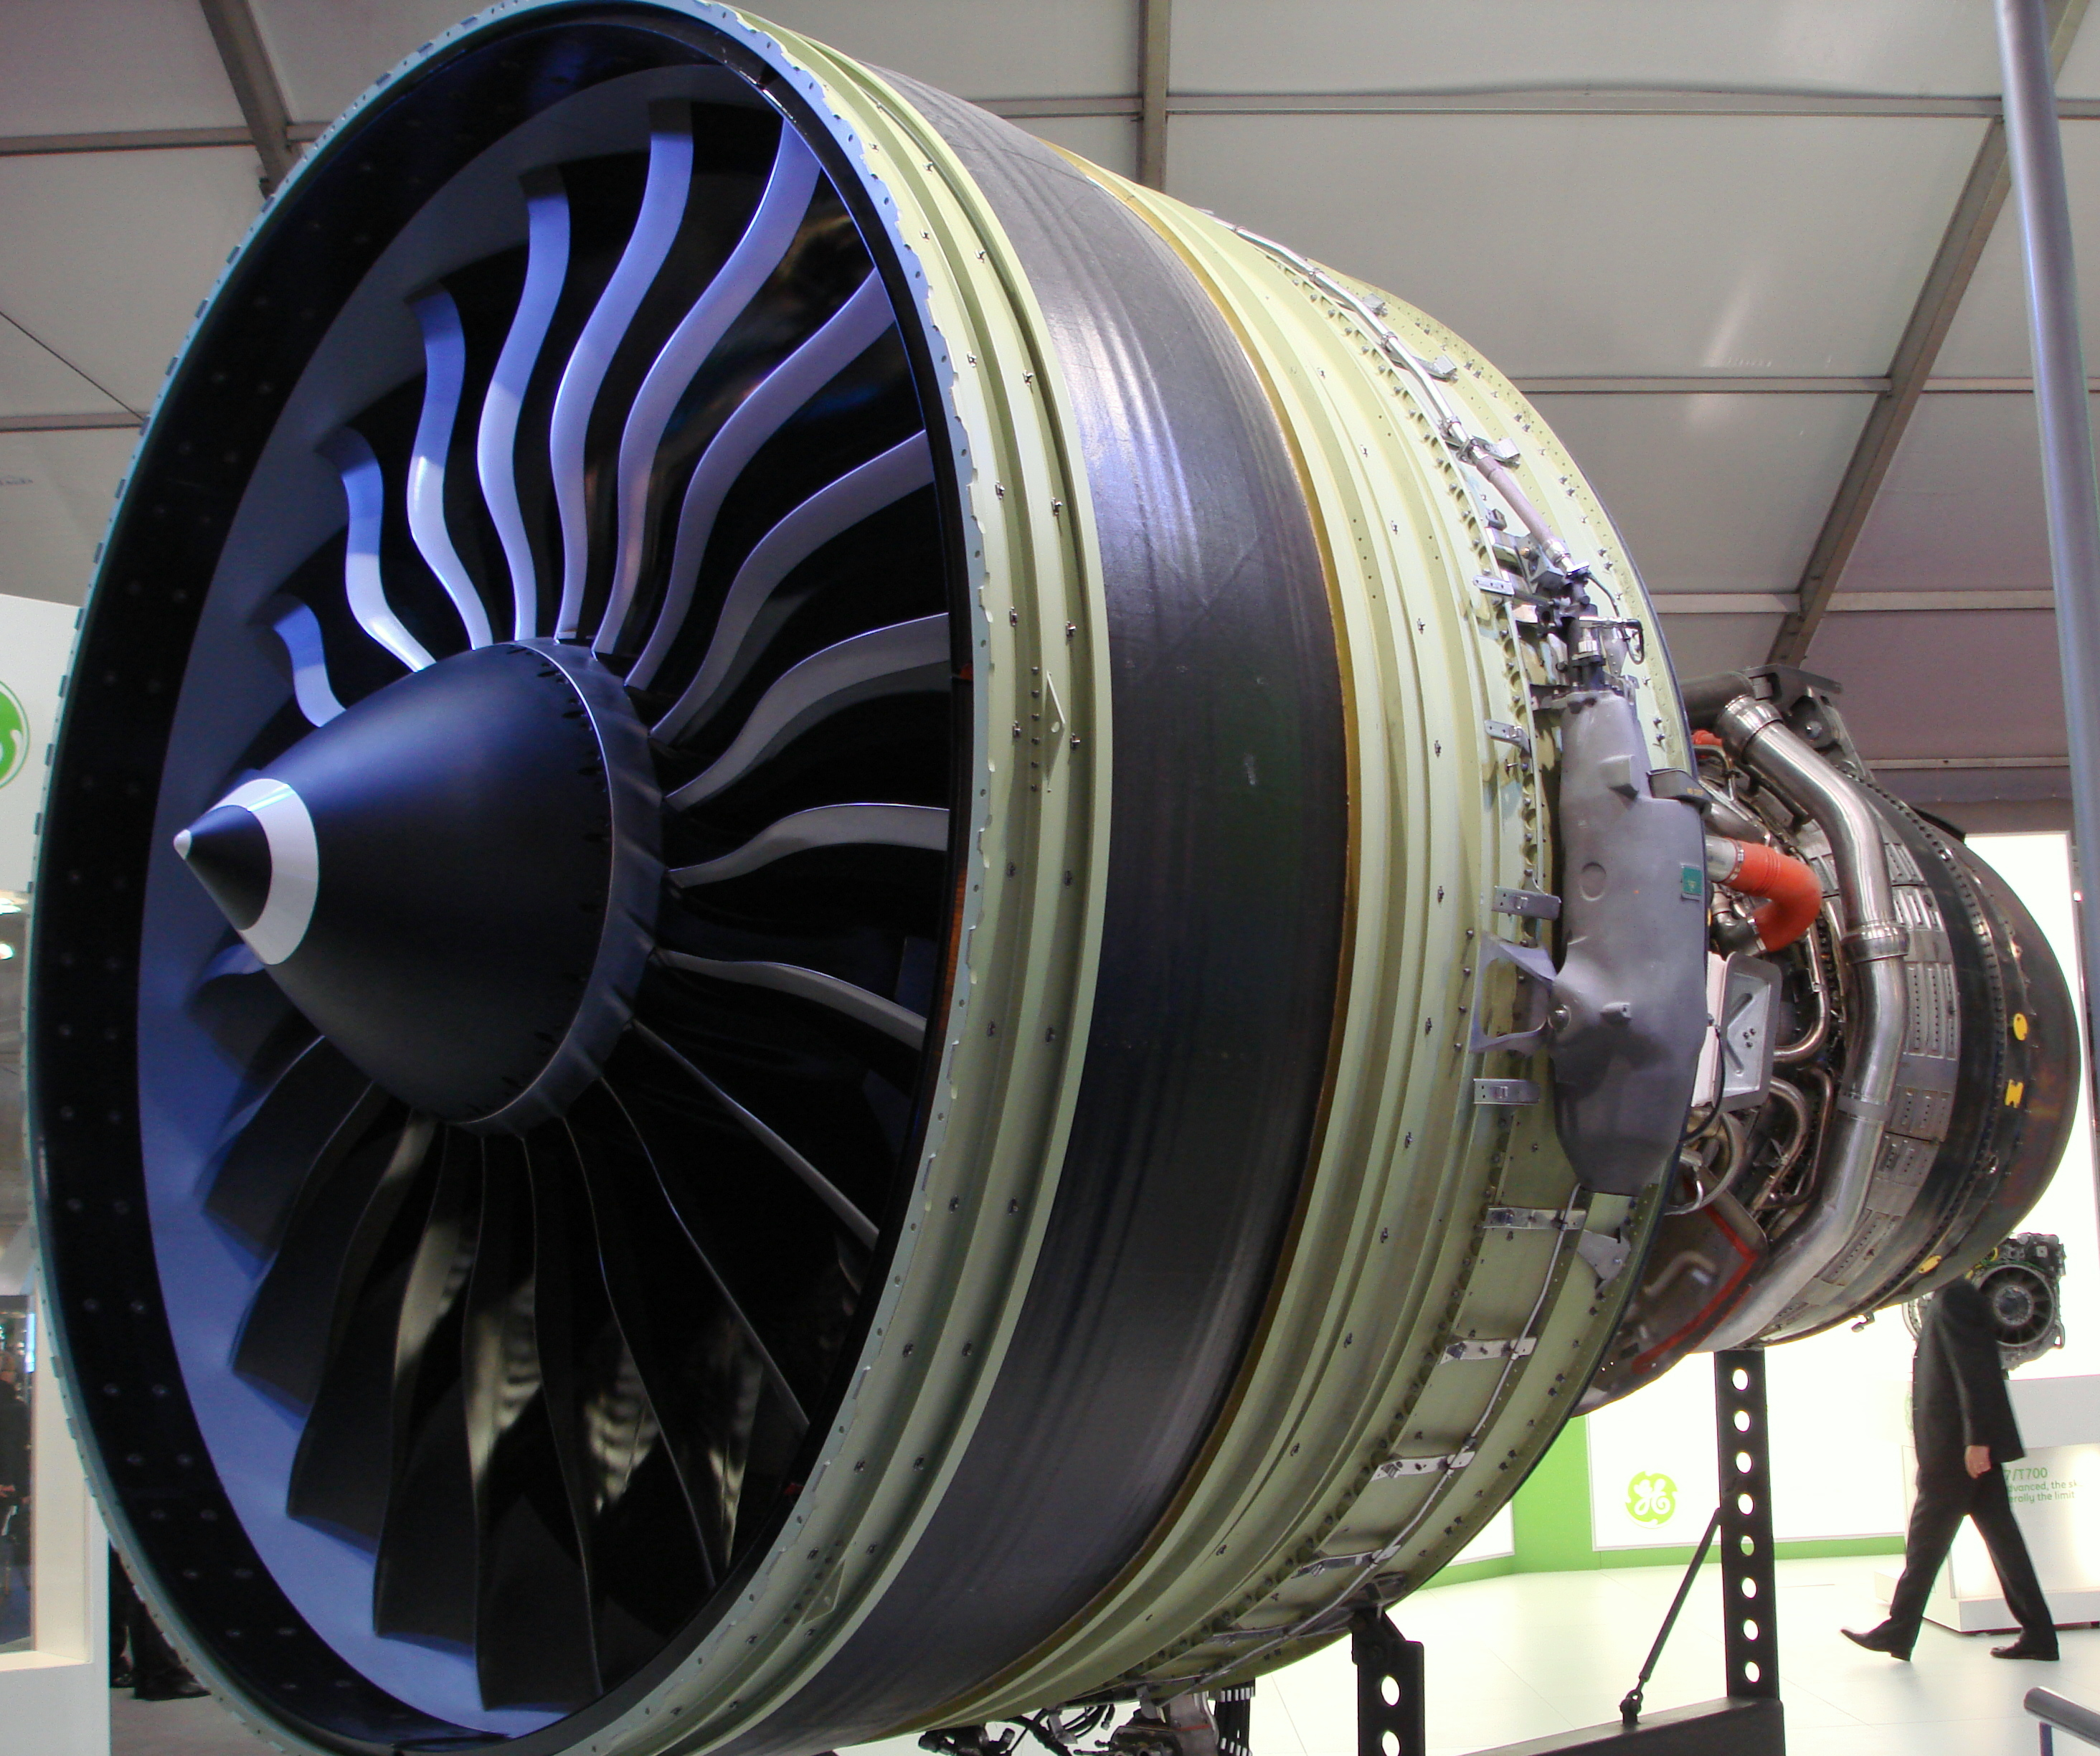
\includegraphics[width=\textwidth]{Sources/Plots_and_Pictures/engine.jpeg}
    \caption{General Electric GE90-94B \autocite{ge90}}
    \label{General_electric}
\end{figure}

\begin{itemize}
    \item Overall Length: 7.283 m
    \item Overall WIdth: 3.871 m
    \item Overall Height: 3.952 m
    \item Dry Weight: 7892 kg
    \item Sea Level Static Thrust (Maximum Continuous): 402.920 kN
    \item Fuel: Jet A
    \item BPR: 8.33
\end{itemize}

\clearpage



\subsection{Assignment 6.3\label{Assignment_6.3}}

\textbf{\textit{Assignment:}} Verify whether or not the propulsive characteristics of the selected 
engine are in line with requirements and with the assumptions of the Conceptual Design \\ \\ \\ 

As mentioned in the previous section \ref{Assignment_6.2}, the thrust requirement is met.\\

Another important parameter is \textit{SFC} (Specific Fuel Consumption), which was initially supposed to be 
$0.478 \ \frac{lb}{lbf \ h}$  ($13.54 \ \frac{mg}{N \ s}$). 

The exact value for this engine wasn't readily available on the internet and different sources
declare different values, which are, however, all comparable to the initial guess.

In addition to this, the \textit{GE90} series have been notorious for having a lower \textit{SFC} 
than their main competitors, at the time of release (November 1995).\\ 

The initial concept design established the presence of twin turboengines, both mounted below the main wing.
This engine is generally used in this configuration with aircrafts of comparable size and performance. \\ 

\begin{figure}[h!]
    \phantomsection
    \centering
    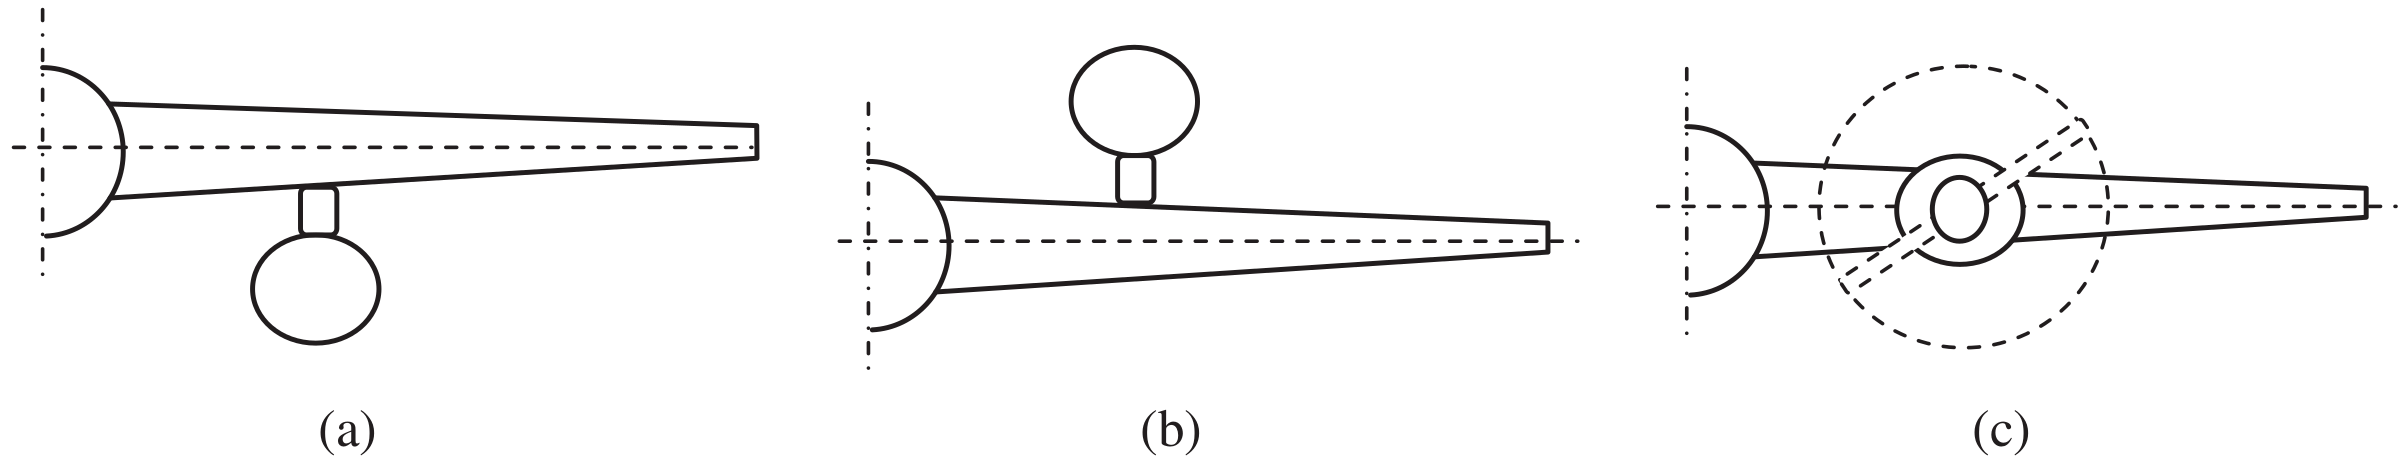
\includegraphics[width=\textwidth]{Sources/Plots_and_Pictures/engine_location.png}
    \caption{The location options for a multi-engine podded configuration with respect to the
    wing: \textbf{(a) Engine under wing}; (b) Engine over wing; and (c) Engine on the wing (prop-driven)}
    \label{engine_location}
\end{figure}


\clearpage




\subsection{Assignment 6.4\label{Assignment_6.4}}

\textbf{\textit{Assignment:}} Create a representative CAD model 
(Mass and Volume should be correct) \\ \\ \\ 

\clearpage





\subsection{Assignment 6.5\label{Assignment_6.5}}

\textbf{\textit{Assignment:}} Evaluate and graphically plot the Take-off run and Take-off distance.
Comments upon the obtained results, also comparing them 
with the requirements set at the beginning of the design process. \\ \\ \\ 

Given the thrust, the number of engines, the friction, the minimum velocity and other inputs, the function \autocite{Airbus_replacement_repo}

\begin{verbatim}
    meaningful_distances_plotter.m
\end{verbatim}

returns:

\begin{itemize}
    \item Ground Roll Distance: 1000.2 m
    \item Takeoff Run: 1350.7 m
    \item Takeoff Distance: 1563.3 m
\end{itemize}

As suggested by the name, the function plots these distances, as well as the actual trajectory of the aircraft. \\ 

\begin{figure}[h!]
    \phantomsection
    \centering
    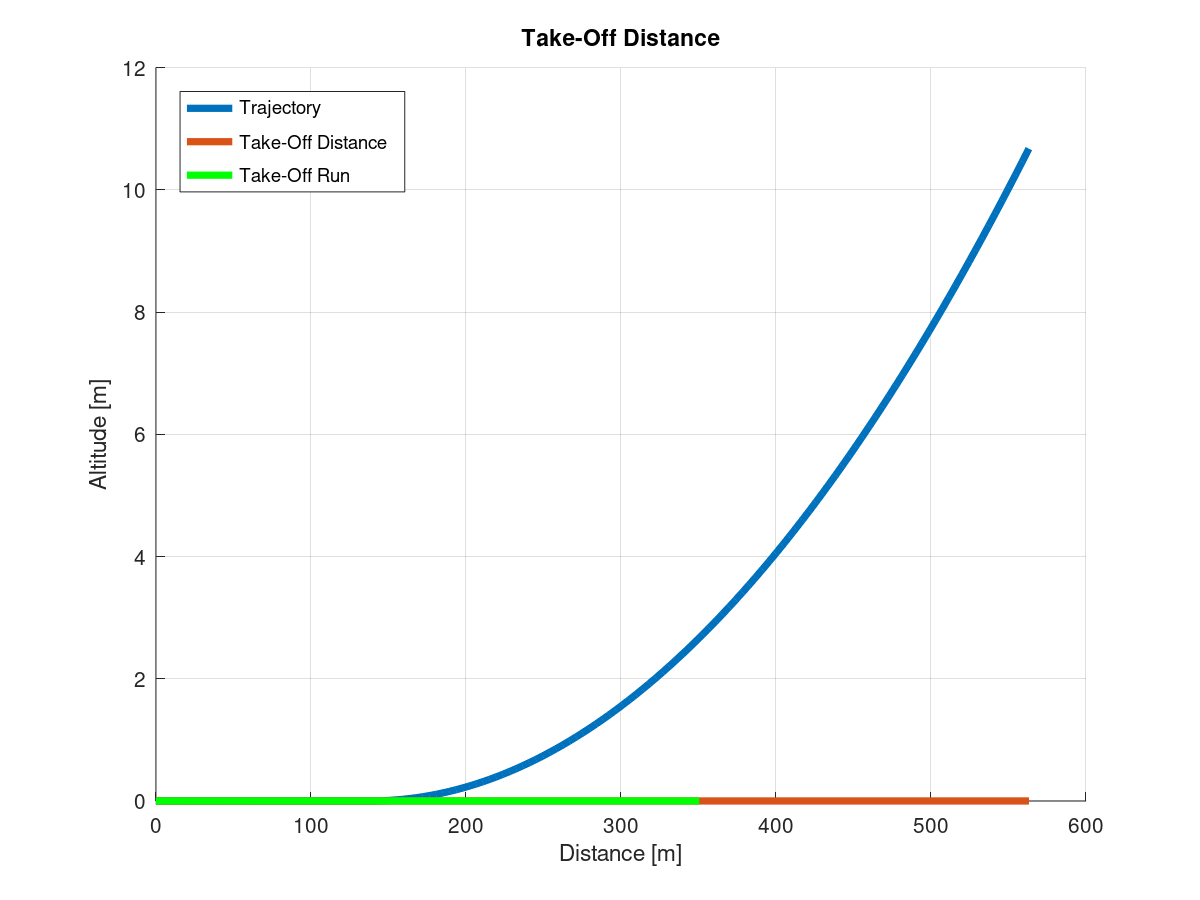
\includegraphics[width=0.9\textwidth]{Sources/Plots_and_Pictures/Distances.png}
    \caption{Meaningful distances}
    \label{distances}
\end{figure}

The only initially guessed value was a ground roll distance of 888 m (\ref{cruise_parameters}), which was clearly lower than this more accurate result. 



\clearpage






\subsection{Assignment 6.6\label{Assignment_6.6}}

\textbf{\textit{Assignment:}} Reproduce the BFL for your case study and plot the graphical solution. 
Comments upon the obtained results, specifically identifying which of the initially 
defined airports can host the operations of this aircraft. \\ \\ \\ 

The function seen in the previous section \ref{Assignment_6.5} plots the \textit{BFL} as well. \\ 

\begin{figure}[h!]
    \phantomsection
    \centering
    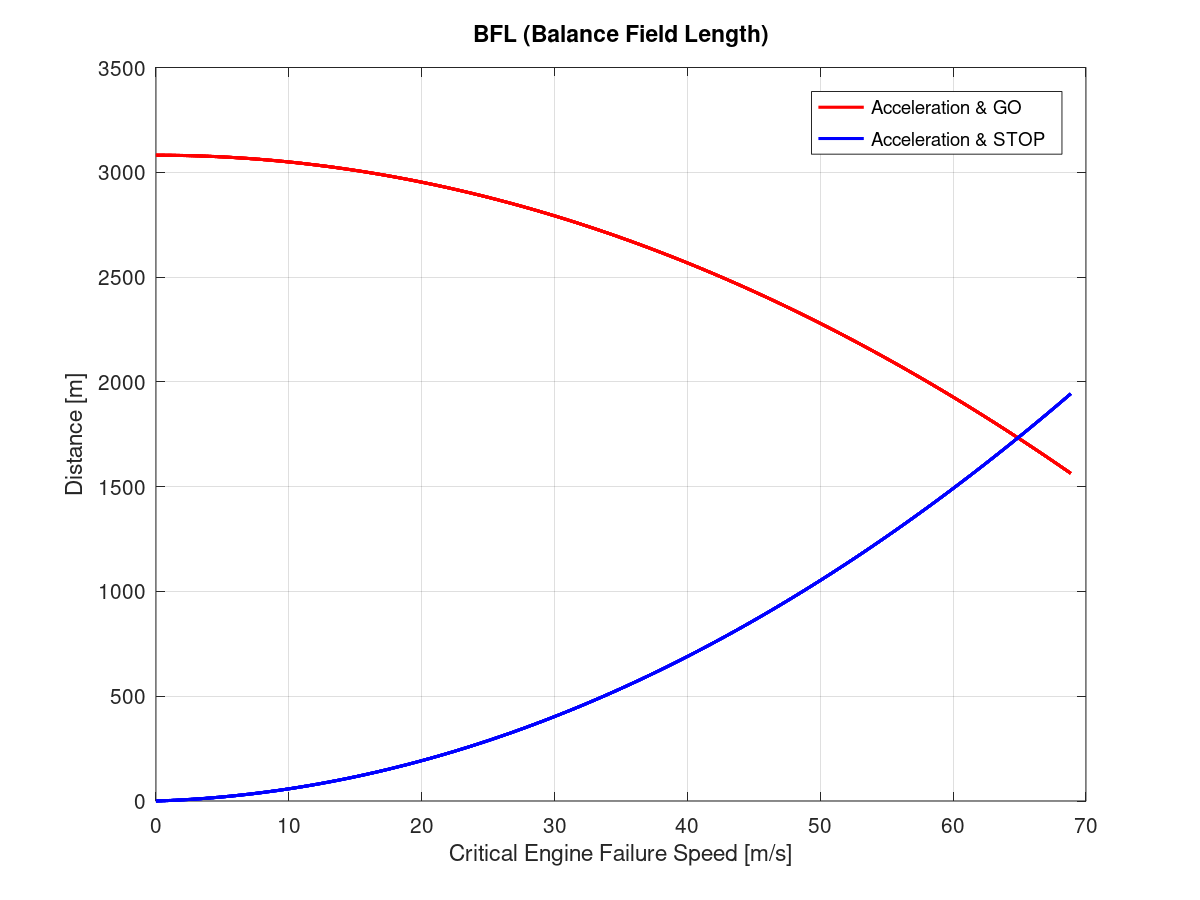
\includegraphics[width=0.9\textwidth]{Sources/Plots_and_Pictures/BFL.png}
    \caption{Balance Field Length}
    \label{BFL}
\end{figure}

All of the cities mentioned in section \ref{Assignment_2.3} have large international airports, that should be 
capable of handling the requirements for the takeoff and landing of the aircraft, with runways usually longer than 3 km. \\

\clearpage






\subsection{Assignment 6.7\label{Assignment_6.7}}

\textbf{\textit{Assignment:}} Create an Assembly file encompassing: 
fuselage, wing, empennages and engines. \\ \\ \\ 

\clearpage

\subsection{Assignment 6.8\label{Assignment_6.8}}

\textbf{\textit{Assignment:}} Create a 3D view dimensioned drawings. \\ \\ \\ 

\clearpage

\subsection{Assignment 6.9\label{Assignment_6.9}}

\textbf{\textit{Assignment:}} dentify the CoG location of the aircraft concept and comments
on its weight and balance characteristics. 
Compare it with the A350 reference configuration. \\ \\ \\ 

\clearpage




\pagebreak
\printbibliography
    
\end{document}

